\documentclass[13pt,onecolumn,a4paper]{article}
\makeatletter
\newcommand*{\rom}[1]{\expandafter\@slowromancap\romannumeral #1@}
\makeatother
\usepackage{epsfig,graphicx,subfig,amsthm,amsmath,accents,cases}
\usepackage{empheq, graphicx, hyperref, physics}
\usepackage{cancel}
\usepackage{floatrow}
\usepackage{amssymb}
\usepackage{MnSymbol,wasysym}
\usepackage{mathtools}
\usepackage{nicefrac,xfrac}
\usepackage{siunitx}
\usepackage{floatrow}
\usepackage{caption}
\usepackage{geometry}
\newcommand{\cmark}{\text{\ding{51}}}%
\newcommand{\xmark}{\text{\ding{55}}}%
\usepackage{amstext} % for \text macro
\usepackage{array}   % for \newcolumntype macro
\newcolumntype{L}{>{$}l<{$}} % math-mode version of "l" column type
\usepackage[table]{xcolor}     
\usepackage{listings}

\definecolor{dkgreen}{rgb}{0,0.6,0}
\definecolor{gray}{rgb}{0.5,0.5,0.5}
\definecolor{mauve}{rgb}{0.58,0,0.82}

\lstset{frame=tb,
	language=Java,
	aboveskip=3mm,
	belowskip=3mm,
	showstringspaces=false,
	columns=flexible,
	basicstyle={\small\ttfamily},
	numbers=none,
	numberstyle=\tiny\color{gray},
	keywordstyle=\color{blue},
	commentstyle=\color{dkgreen},
	stringstyle=\color{mauve},
	breaklines=true,
	breakatwhitespace=true,
	tabsize=3
}
\usepackage[extrafootnotefeatures]{xepersian}
\settextfont[Scale=0.9]{Yas}
\setlatintextfont[Scale=0.83]{Times New Roman}
\ExplSyntaxOn \cs_set_eq:NN \etex_iffontchar:D \tex_iffontchar:D \ExplSyntaxOff
\setmathdigitfont{Yas}
\title{بازآفرینی مقاله\\ \lr{Nonlinear asset-price dynamics and stabilization policies}}
\author{عرفان رهبری - صالح شاملو احمدی
}
\date{تیرماه ۰۲}
\hypersetup{colorlinks=true, citecolor=cyan, urlcolor=blue}
\newfloatcommand{capbtabbox}{table}[][\FBwidth]

\usepackage{blindtext}
\makeatletter
\newcommand{\Spvek}[2][r]{%
	\gdef\@VORNE{1}
	\left(\hskip-\arraycolsep%
	\begin{array}{#1}\vekSp@lten{#2}\end{array}%
	\hskip-\arraycolsep\right)}

\def\vekSp@lten#1{\xvekSp@lten#1;vekL@stLine;}
\def\vekL@stLine{vekL@stLine}
\def\xvekSp@lten#1;{\def\temp{#1}%
	\ifx\temp\vekL@stLine
	\else
	\ifnum\@VORNE=1\gdef\@VORNE{0}
	\else\@arraycr\fi%
	#1%
	\expandafter\xvekSp@lten
	\fi}
\makeatother

\begin{document}
	\maketitle

	\section{مقدمه}
	پدیده‌های موجود در بازارهای اقتصادی مانند حباب، افت و خیزهای شدید و غیر منتظره قیمت و ... از مسائل مهم برای بررسی در علم اقتصاد هستند. برای شناخت و بعضا جلوگیری از رخداد این پدیده‌ها به ساخت و بررسی مدل‌های ریاضیاتی نیاز داریم. از آنجا که پدیده‌های مشهود در این سیستم‌ها به نظر خطی نیستند سراغ ساختن مدل‌های غیر خطی می‌رویم:
	
	
	
	\section{مدل}
	\subsection{رفتار سرمایه‌گذار}
	برای ساده سازی مدل از این فرض استفاده می‌کنیم که دو کالا یکی با ریسک و یکی بدون ریسک داریم (قیمت کالای بدون ریسک با قیمت بنیادی‌اش برابر است). اگر عامل\footnote{\lr{agent}} 
	$i$
	ام در زمان 
	$t$ 
	میزان 
	$Z_t^i$
	از کالای دارای ریسک داشته باشد و ثروتش هم در این زمان 
	$W_t^i$ 
	باشد، برای ثروتش در یک قدم جلوتر داریم:
	$$W_{i,t+1}=(1+r)W_{i,t}+\left(P_{t+1}+D_{t+1} - (1+r)P_t\right)Z_{i,t}$$
	که در آن 
	$D$
	سود او و 
	$r$ 
	نرخ بهره خواهد بود. به این معنا که افزایش ثروت فرد در این بازه زمانی به چند فاکتور وابسته است:\\
	
	۱)		افزایش ثروتش توسط نرخ بهره\\
	
	۲) 	پولی که از فروش کالای ریسکی در پایان این بازه بدست می‌آورد\\
	
	۳) 	سود حاصل از این کالا\\
	
	۴) 	میزان پولی که اگر کالا را در ابتدای بازه فروخته بود بدست می‌آورد با احتساب نرخ بهره\\
	
یک فرض مهم در این مدل این است که هر عامل در این مدل صرفا قصد دارد تا ثروتش را در یک قدم جلوتر بیشینه کند. یعنی هر عامل می‌خواهد. یعنی او با تغییر میزان دارایی‌اش از کالای دارای ریسک قصد دارد تا مطلوبیتش در زمان جلوتر بیشینه شود. تابعی که برای مطلوبیت در این مدل استفاده می‌شود:
$$U_i(W)=-e^{-\alpha_iW}$$
که 
$\alpha_i$ 
مثبت و نشانگر ریسک گریزی \footnote{\lr{risk aversion}} عامل $i$ام است. از آنجا که از مقادیری که اندیس $t+1$ دارند اطلاعی نداریم، آنها را تصادفی در نظر میگیریم. در نتیجه برای یافتن عبارت بیشینه و با بکارگیری تابع بالا خواهیم داشت:
$$\max_{Z_{i,t}}\mathbb{E}_{i,t}\left[U_i\left(W_t^i\right)\right]=\max_{Z_{i,t}}\left[\mathbb{E}_{i,t}(W_t^i)-\frac{\alpha_i^2}{2}\mathbb{V}_{i,t}(W_t^i)\right]$$
که در آن 
$\mathbb{E}_{i,t}$ 
مقدار چشمداشتی و 
$\mathbb{V}_{i,t}$ 
واریانس شرطی است. در نتیجه تقاضا برای کالای ریسکی:
$$Z_{i,t}=\frac{\mathbb{E}_{i,t}\left(P_{t+1}+D_{t+1}-(1+r)P_t\right)}{\alpha_i\mathbb{V}_{i,t}\left(P_{t+1}+D_{t+1}-(1+r)P_t\right)}$$
$$\Rightarrow Z_{i,t}=\frac{\mathbb{E}_{i,t}\left(P_{t+1}\right)+\mathbb{E}_{i,t}\left(D_{t+1}\right)-(1+r)P_t}{\alpha_i\mathbb{V}_{i,t}\left(P_{t+1}+D_{t+1}\right)}$$
برای ادامه چهار فرض در نظر میگیریم:\\
	
	۱)		چشمداشت تمام سرمایه‌گذاران از سود برابر $\bar{D}$ است\\
	
	۲) 	باور تمام سرمایه‌گذاران از واریانس برابر $\sigma_2^R$ است\\
	
	۳) 	ریسک گریزی همه‌ی آن ها برابر $\alpha$ است.\\
	
	۴) 	میانگین چشمداشت سرمایه‌گذاران از قیمت برابر $\mathbb{E}_{t}\left(P_{t+1}\right)$ است.\\
	
	با وجود فرض‌های بالا می‌توانیم تقاضا را برای کالای ریسکی را بدست آوریم و سپس آن را بهنجار کنیم (مانند روش میدان میانگین در مکانیک آماری):
	$$Z_{S,t}=\frac{1}{N}\sum_{i}^{N}Z_{i,t}=\frac{\mathbb{E}_{t}\left(P_{t+1}\right)+\bar{D}-(1-r)P_t}{\alpha\sigma_2^R} $$
	برای حساب کردن میانگین چشمداشت سرمایه‌گذاران از میزان قیمت فرض می‌کنیم کسر $N_C$ از آنها از تحلیل فنی\footnote{\lr{technical}} و باقی آن‌ها ($N_F$) از تحلیل بنیادی\footnote{fundamental} بهره میگیرند. در نتیجه:
	$$\mathbb{E}_{t}\left(P_{t+1}\right)=N_{C,t}\mathbb{E}_{C,t}\left(P_{t+1}\right)+N_{F,t}\mathbb{E}_{F,t}\left(P_{t+1}\right)$$
حال باید مدل‌هایی برای شیوه‌ی تحلیل‌های تکنیکی و بنیادی از قیمت ارائه کنیم. تفاوت اصلی این دو گروه این است که یکی انتظار دارد فاصله‌ی بین قیمت بنیادی و قیمت بازار این کالا ها کم شود و دیگری انتظار دارد این فاصله زیاد شود. این انتظارات با معادلات زیر بیان می‌شوند:
\begin{empheq}[left=\empheqlbrace]{align*}
	\mathbb{E}_{C,t}\left(P_{t+1}\right)= P_{t-1} + \chi \left(P_{t-1}-F\right)\\
	\mathbb{E}_{F,t}\left(P_{t+1}\right)= P_{t-1} - \phi \left(P_{t-1}-F\right)
\end{empheq}
	که در آن $F$ قیمت بنیادی کالا است که با رابطه‌ی $F=\nicefrac{\bar{D}}{r}$ مشخص می‌شود و همچنین هر دو ثابت $\chi$ و $\phi$ مثبت و همچنین $\phi$ کوچکتر یا مساوی واحد است. تحلیل‌های بالا به این جهت کارآمد است که اندیس‌های مربوط به آینده را از بین می‌برد. حالا سرمایه گذاران باید بین این دو تحلیل یکی را انتخاب کنند؛ تمایل برای انتخاب هر کدام از این تحلیل‌ها به سود حاصل از آن‌ها در مرحله قبل بستگی دارد:
\begin{empheq}[left=\empheqlbrace]{align*}
	A_{C,t}&=\left(P_{t-1}+D_{t-1} - (1+r)P_{t-2}\right)Z_{C,t-2}\\
	A_{F,t}&=\left(P_{t-1}+D_{t-1} - (1+r)P_{t-2}\right)Z_{F,t-2}-\kappa
\end{empheq}
	که در آن:
$$Z_{C,t-2}=N_{C,t-2}Z_{S,t-2}\qquad\&\qquad Z_{F,t-2}=N_{F,t-2}Z_{S,t-2}$$
در رابطه با معادلات بالا تمایل برای تحلیل بنیادی کمتر است چرا که یافت  اطلاعات در باره قیمت بنیادی هزینه بر است و همچنین چون تحلیل تکنیکی آسان‌تر است جاذبه‌ی بیشتری دارد؛ ثابت $\kappa$ برای لحاظ این استدلال‌ها لحاظ شده است. حالا می‌توانیم کسر سرمایه گذاران با هر تحلیل را بیابیم؛ توزیع سرمایه‌گذاران در این مدل مشابه توزیع بولتزمن خواهد بود:

	\begin{empheq}[left=\empheqlbrace]{align*}
		N_{C,t}&=\frac{\beta A_{C,t}}{\beta A_{C,t}+\beta A_{F,t}}\\
		N_{F,t} &=A_{F,t}=\frac{\beta A_{F,t}}{\beta A_{C,t}+\beta A_{F,t}}
	\end{empheq}
	که در آن هر چه پارامتر $\beta$ بزرگ‌تر باشد سرمایه‌گذاران راحت‌تر تحلیل خود را از بازار تغییر می‌دهند. 
	\subsection{رفتار قدرت مرکزی}
	رفتار قدرت مرکزی\footnote{\lr{central authority}} (که در ادامه آن را دولت می‌نامیم) در بازار برای جلوگیری از ناپایداری بازار رخ می‌دهد. استراتژی مورد بررسی ما ترکیبی از دو استراتژی است؛ اول اگر قیمت رو به افزایش(کاهش) باشد دولت اقدام به فروش(خرید) از کالای دارای ریسک می‌کند و دوم دولت سعی می‌کند قیمت را به سمت قیمت بنیادی هدایت کند:
	$$Z_{G,t}=-m\left(P_{t-1}-P_{t-2}\right)-d\left(P_{t-1}-F\right)$$
	ضرایب مورد استفاده هر دو مثبت و بیانگر ترجیح دولت در استفاده از هر یک استراتژی‌ها هستند.\\
	تا اینجا دو نوع از تقاضا کننده‌گان کالای ریسک‌دار را بررسی کردیم. برای تکمیل، به بررسی دو نوع دیگر نیاز داریم؛ اول سرمایه‌گزاران طولانی مدت\footnote{\lr{long-term investors}} که تقاضای آن‌ها در طی زمان ثابت است:
	$$Z_{I,t}=\bar{Z}_{I}$$
	
	 و دوم سرمایه‌گذاران نقدینه\footnote{\lr{liquidity investors}} که تقاضای آن‌ها تصادفی است و آن را با تابع توزیع نرمال مدل می‌کنیم:
	$$Z_{L,t}\approx N(0,\sigma_L^2)$$
	 حالا تقاضای کل را داریم:
	 $$Z_{t}=Z_{S,t}+Z_{G,t}+Z_{I,t}+Z_{L,t}$$
	از طرفی در تعادل بازار عرضه‌ی این کالا با تقاضا برابر و همچنین برابر با تقاضای سرمایه‌گذاران طولانی مدت است. در نتیجه برای تحولات قیمت خواهیم داشت:
	$$P_t=\frac{\mathbb{E}_{t}\left(P_{t+1}\right)+\bar{D}+\alpha\sigma_R^2(Z_{G,t}+Z_{L,t})}{1+r}$$
	\pagebreak
	\section{تحلیل سیستم}
	\begin{itemize}
		\item 
		اگر چشمداشت سرمایه گذاران از قیمت خیلی بالا باشد قیمت بالا می‌رود.
		\item
		یکی از نقطه ثابت‌های این نگاشت نقطه‌ی $P_1=F$ است
		\begin{itemize}
			\item اینکه دولت کدام استراتژی را در پیش بگیرد تاثیری در این نقطه نخواهد داشت.
			
			\item توزیع جمعیت سرمایه‌گذاران در این نقطه بین دو تحلیل به صورت زیر خواهد بود:
			
			 $N_{1C}=\left(1+\exp(-\beta\kappa)\right)^{-1}$ \qquad $N_{1F}=\left(1+\exp(\beta\kappa)\right)^{-1}$

		\end{itemize}
	\item 
	در نقطه‌ی 
	$N_{1C}\chi+N_{1F}\phi=r+\alpha\sigma_R^2d$ 
	یک دوشاخگی از جنس چنگال \footnote{\lr{pitchfork}} رخ می‌دهد
	
			\begin{itemize}
				\item 
				اگرچه استراتژی اول دولت («خرید در هنگام نزول و فروش در هنگام صعود» که مربوط به پارامتر $m$ در مدل است) در رخدادن این دوشاخگی و کنترل آن بی تاثیر است، با استفاده از استراتژی دوم می‌تواند اقدام به جلوگیری از این دوشاخگی و یا حتی معکوس کردن این فرایند آن کند و دوشاخگی را از  بین ببرد(مربوط به پارامتر $d$).
				
			\end{itemize}
		\item 
		بعد از رخدادن دوشاخگی، دو نقطه ثابت پایدار جدید داریم:
	$$P_{2,3}=P_1\pm\sqrt{\frac{2\alpha\sigma_R^2\left(\nicefrac{1}{2}\beta\kappa+\tanh[-1](N_{F2,3}-N_{C2,3})\right)}{r\beta\left(\chi+\phi\right)}}$$
		که در آن:
		$$ N_{F2,3}=\frac{\phi -r- \alpha\sigma_R^2d}{\chi + \phi} \quad\&\quad N_{C2,3}=\frac{\phi +r+ \alpha\sigma_R^2d}{\chi + \phi}$$
		
\item 
از طرفی اگر در معادلات بالا $\chi$ را به اندازه کافی بزرگ کنیم، نقاط $P_{2,3}$ پایداری خود را از دست می‌دهند و یک دو شاخگی جدید رخ می‌دهد؛ دوشاخگی \footnote{Neimark–Sacker bifurcation}\lr{NSB}	



\end{itemize}
\section{بررسی عددی}
با توجه به معدلاتی که بدست آمد، با پارامترهای زیر شروع به حل عددی معادلات میکنیم:
$$\alpha=\sigma_R^2=\phi=\kappa=\bar{D}=1$$
$$\sigma_L=0,\;m=0,\;d=0$$
$$r=0,1,\; \chi=0.2,\;\beta=3.6$$

	
	
	\begin{figure}[H]
		\centering
		\sidesubfloat[]{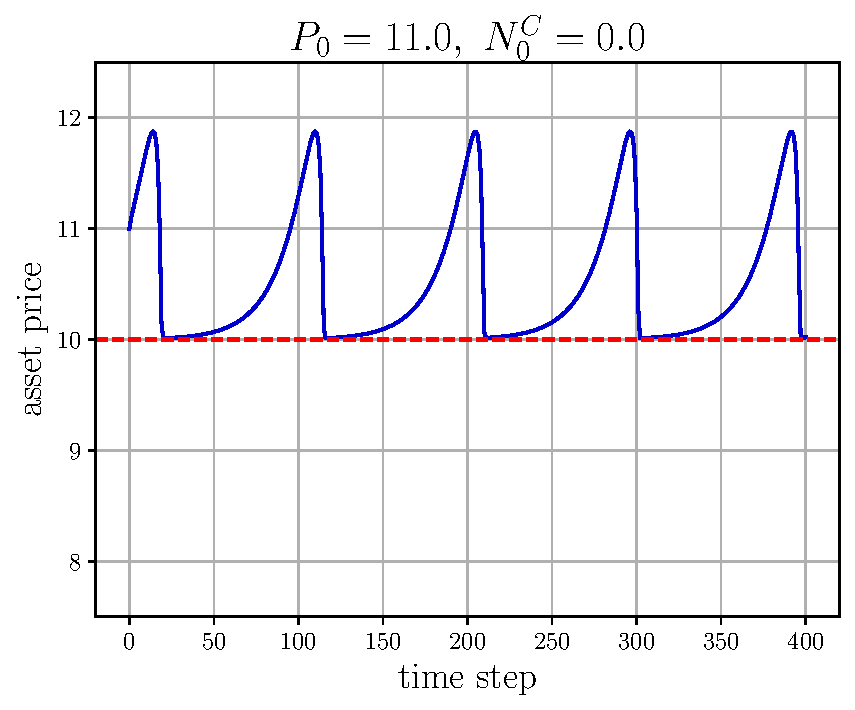
\includegraphics[width=0.4\textwidth]{../results/no-intervention-1.pdf}\label{fig:a}}
		\hfil
		\sidesubfloat[]{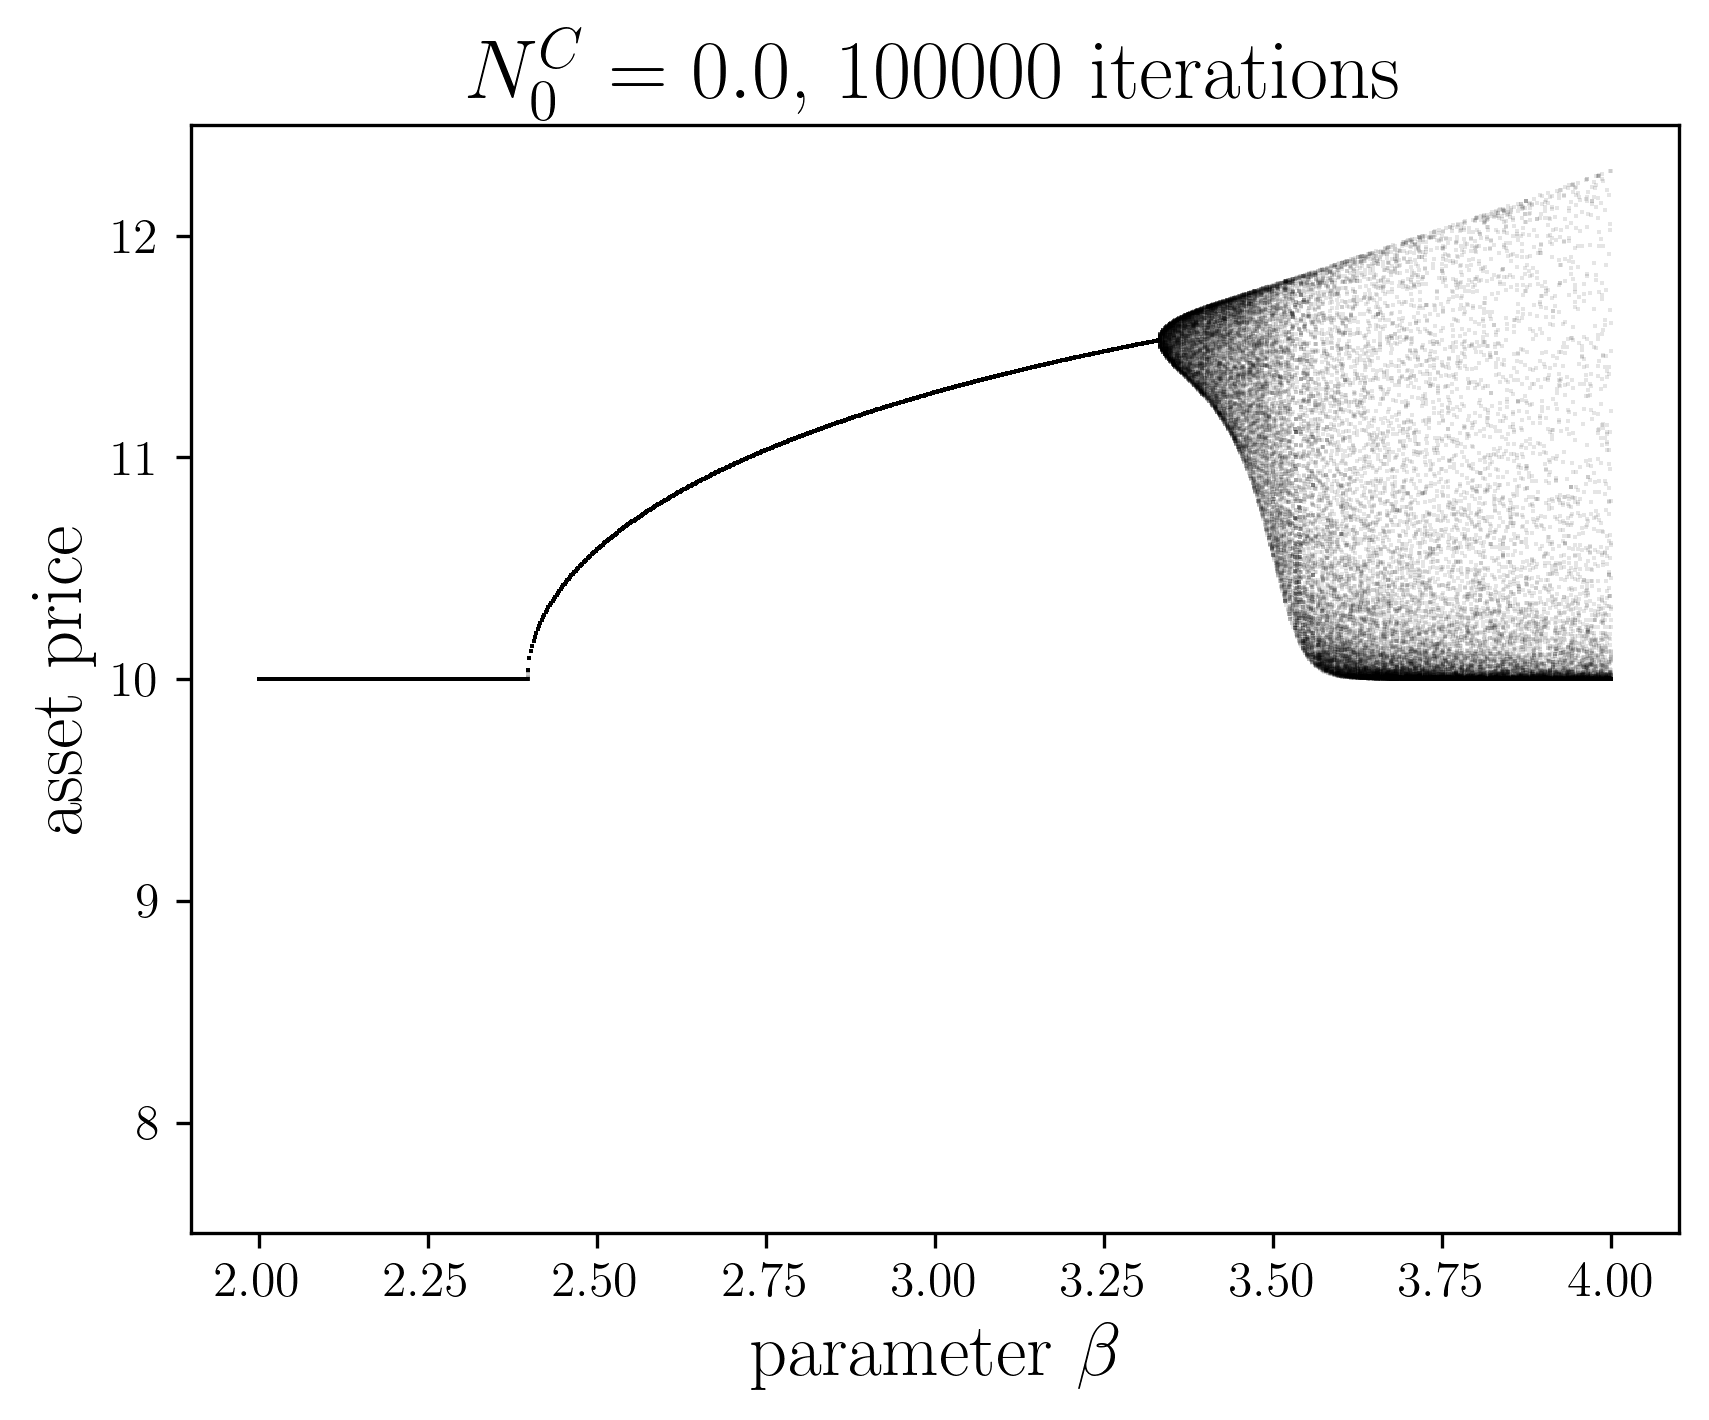
\includegraphics[width=0.4\textwidth]{../results/no-intervention-bifurcation-1.png}\label{fig:b}}
		
		\medskip
		\sidesubfloat[]{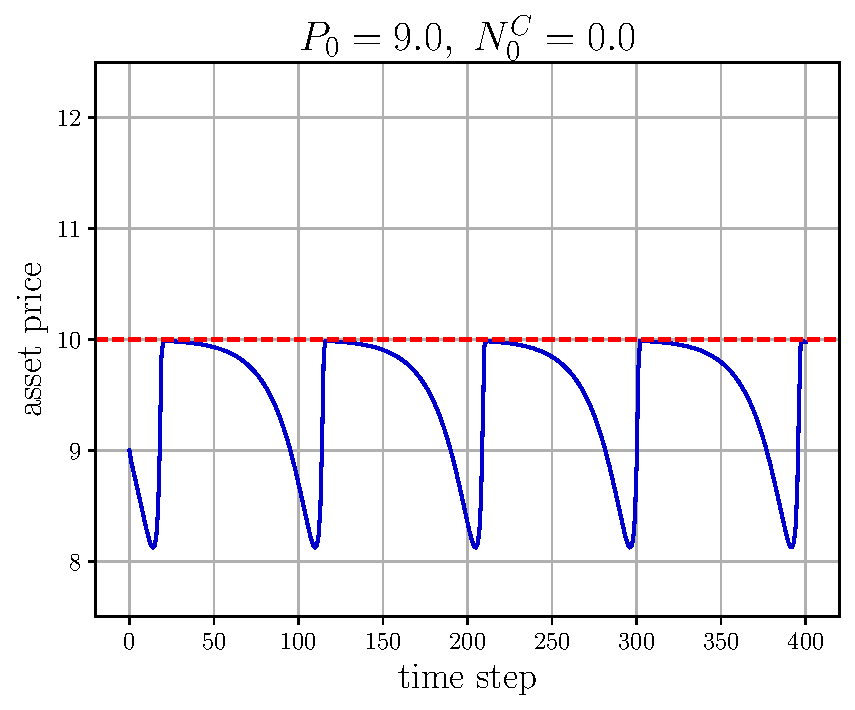
\includegraphics[width=0.4\textwidth]{../results/no-intervention-2.pdf}\label{fig:c}}
		\hfil
		\sidesubfloat[]{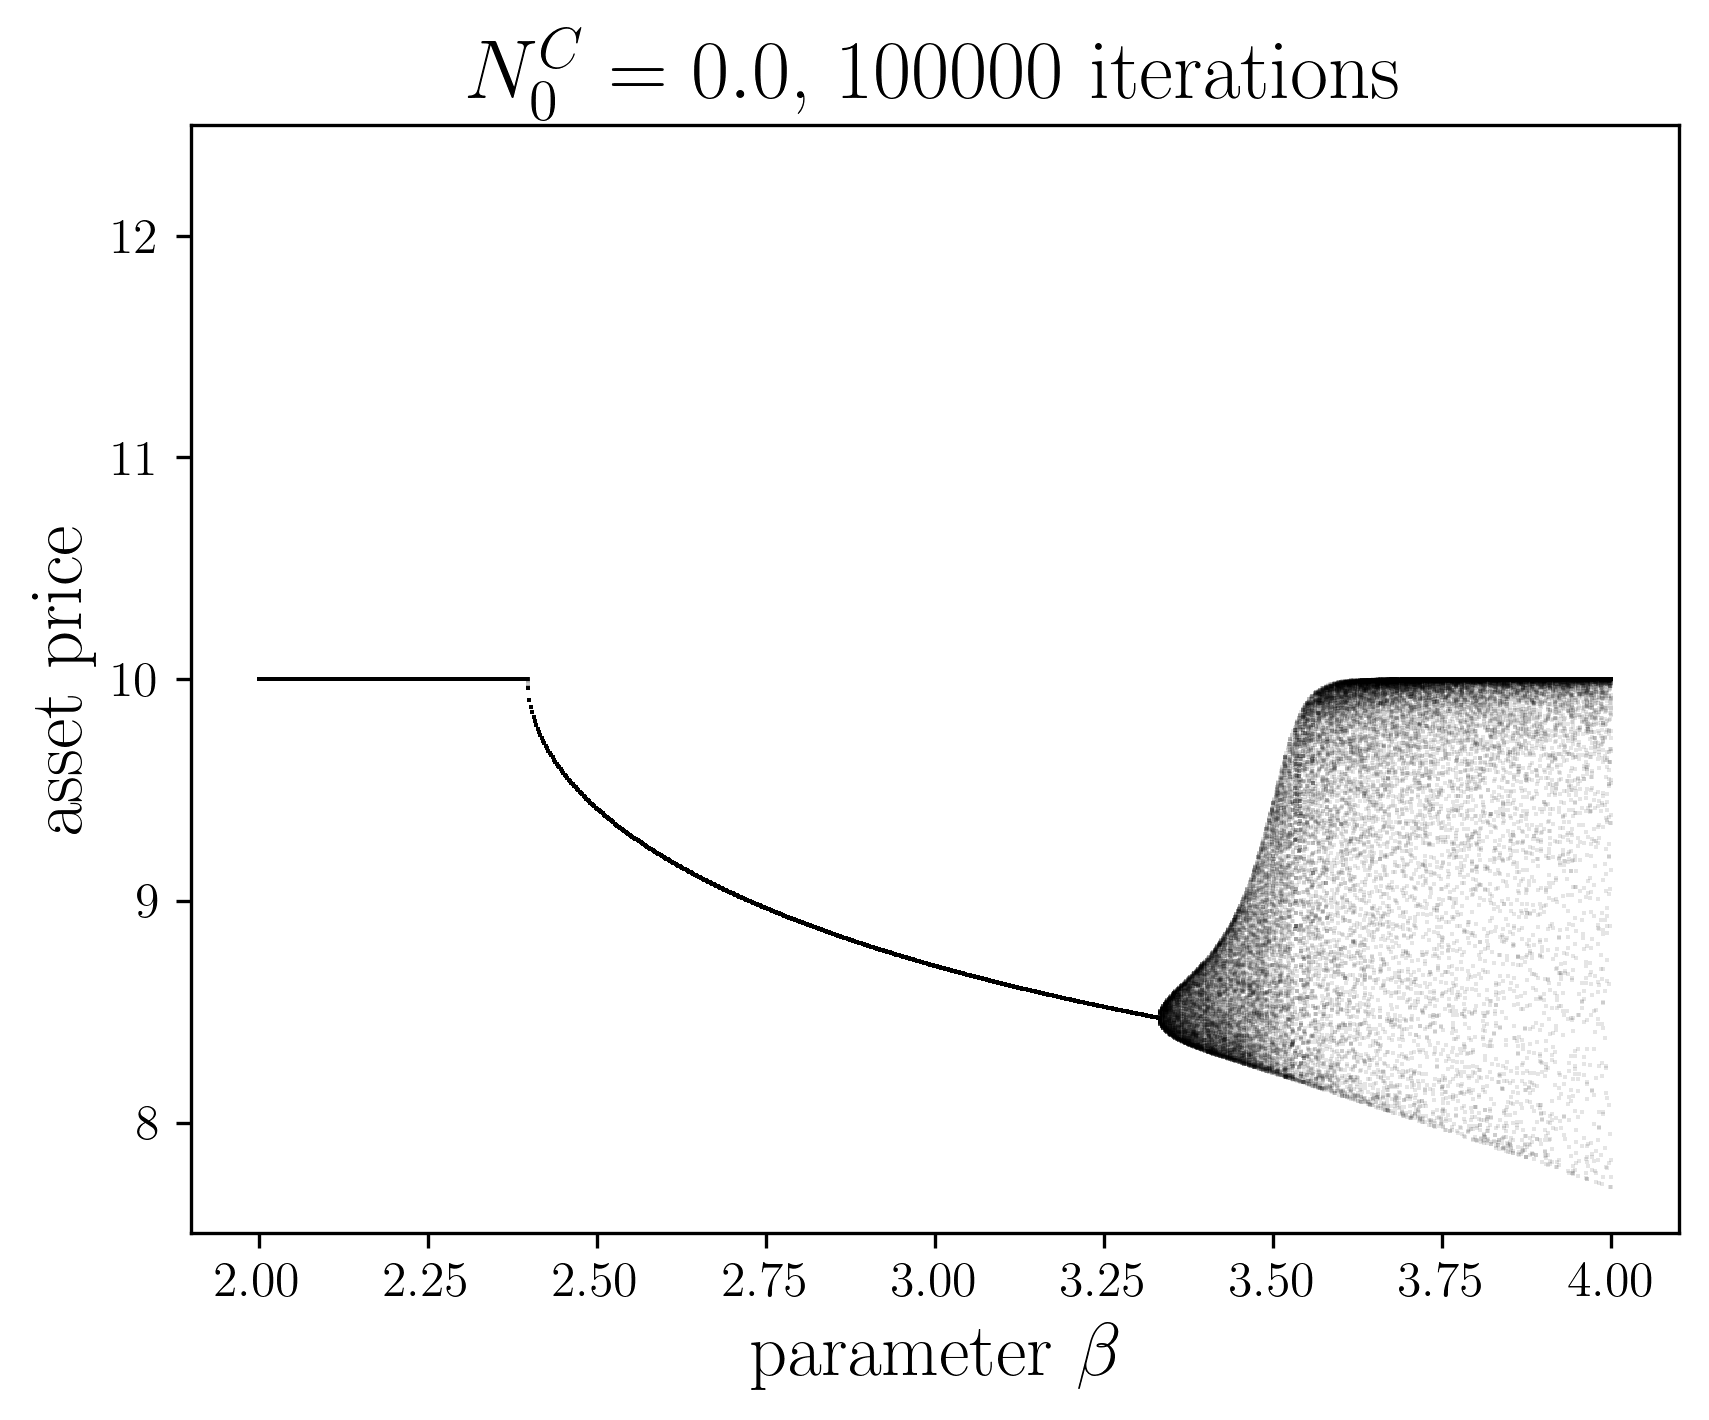
\includegraphics[width=0.4\textwidth]{../results/no-intervention-bifurcation-2.png}\label{fig:d}}
		
		\medskip
		\sidesubfloat[]{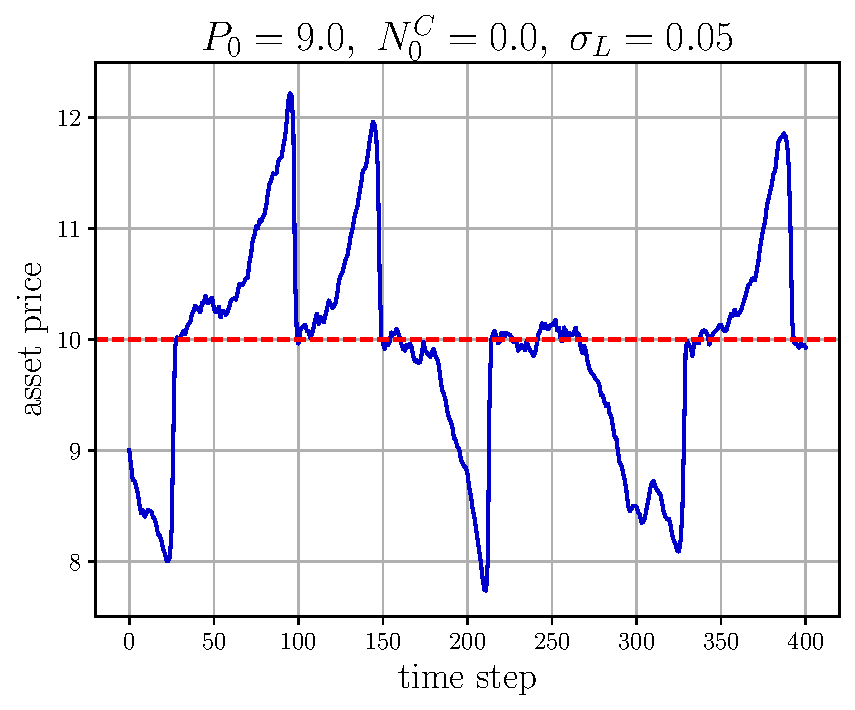
\includegraphics[width=0.4\textwidth]{../results/no-intervention-stochastic.pdf}\label{fig:e}}
		\hfil
		\sidesubfloat[]{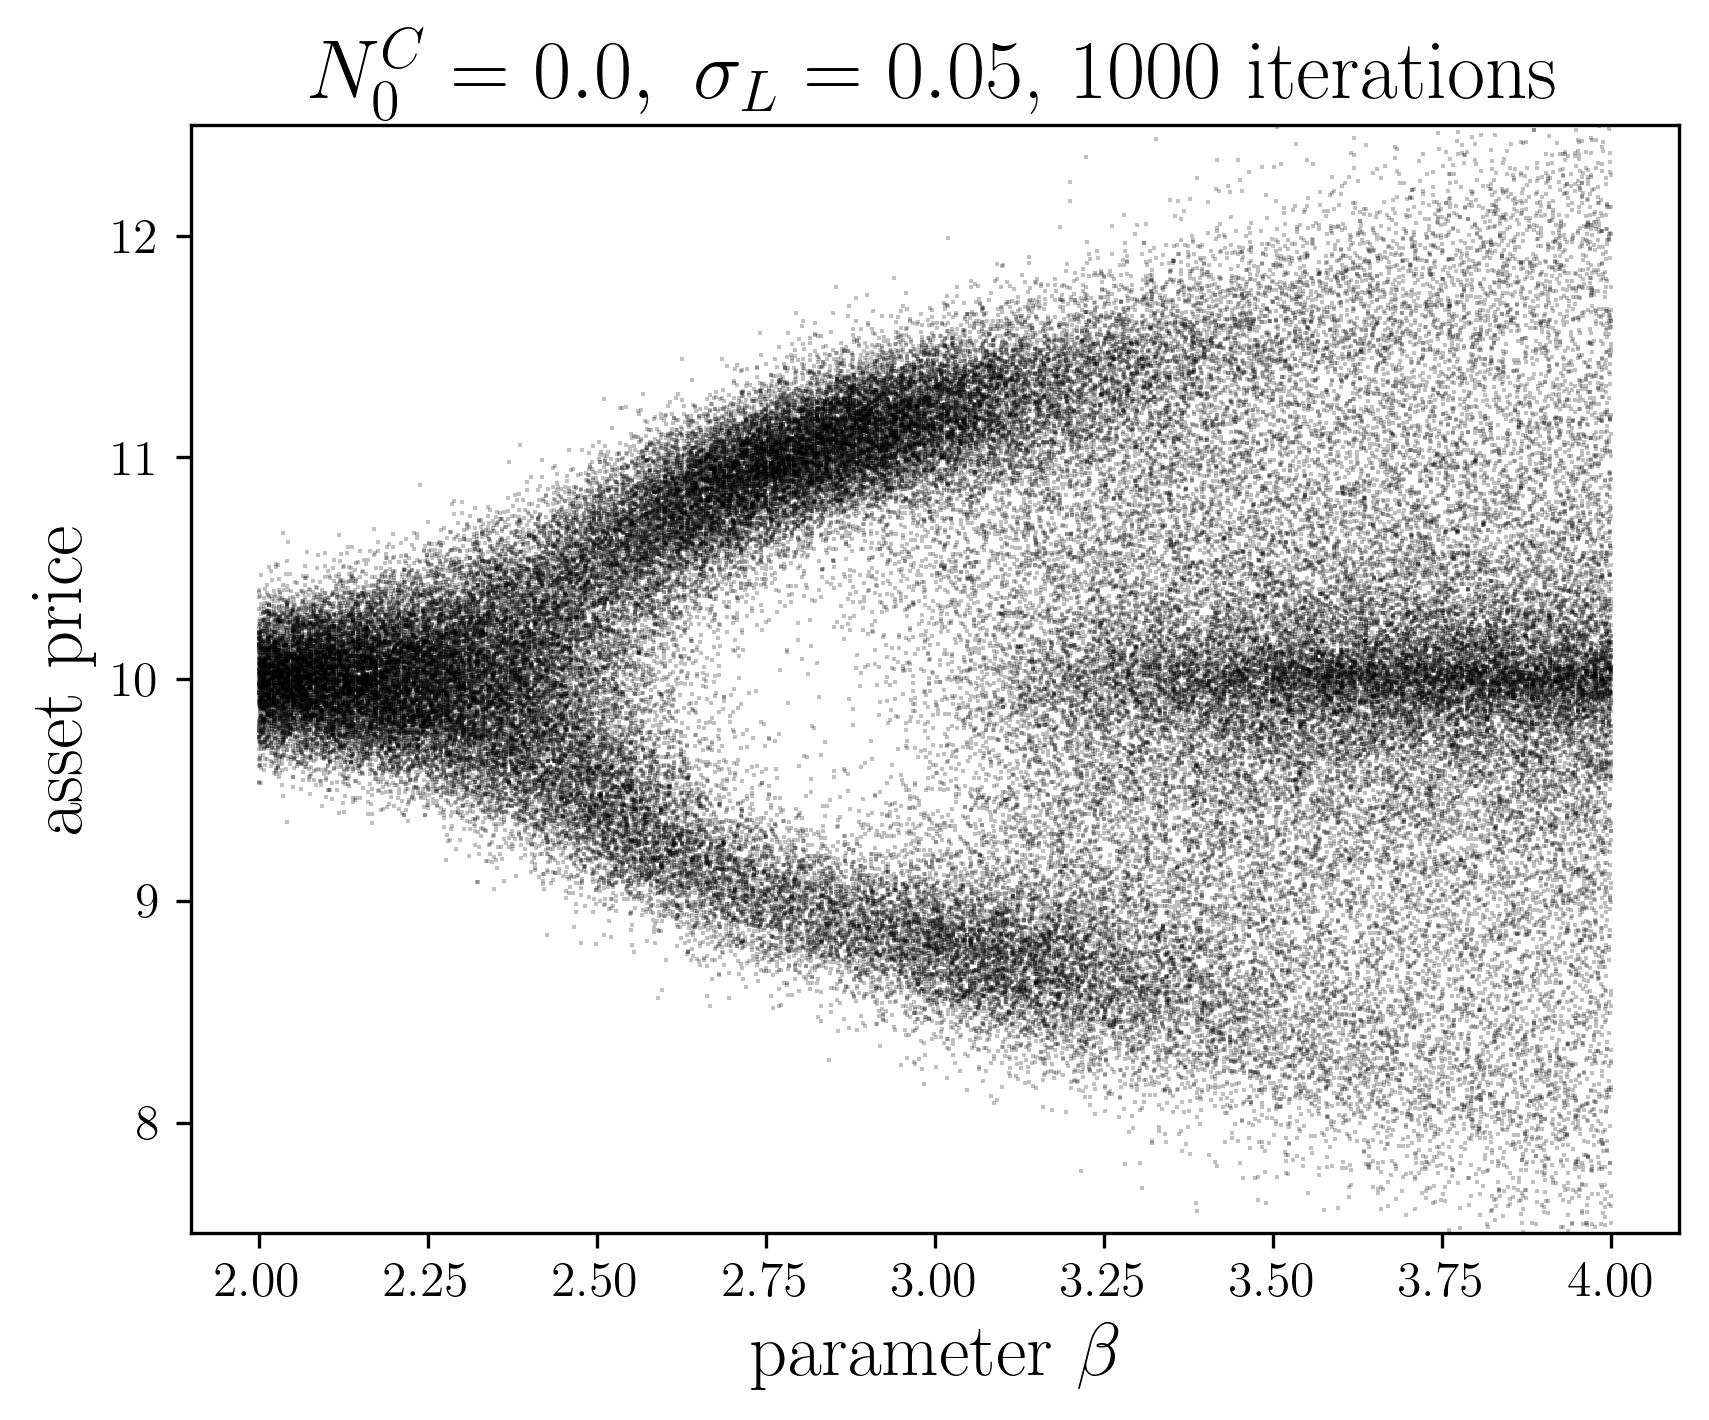
\includegraphics[width=0.4\textwidth]{../results/no-intervention-bifurcation-stochastic.png}\label{fig:f}}
		\caption{نوسانات و تغییرات بازار درغیاب دولت }
		\label{fig:myfigure}
	\end{figure}
در شکل ۱ به بررسی بازار تنظیم نشده می‌پردازیم؛ در این بازار که برای مدت ۴۰۰ قدم زمانی اجرا شده به نظر می‌اید برای مقادیر کم $\beta$ بازار وارد فاز آشوب نمی‌شود (ب و د) و شاید حتی بتوان گفت که پایدار است اما به محض آنکه کمی عدم قطعیت ($\sigma_L^2=\nicefrac{1}{400}$) حالت‌های پایدار، شروع به ناپایدار شدن می‌کند و خم پایدار تبدیل به ناحیه پایدار می‌شود (و) و در ادامه این نواحی به قدری پهن می‌شوند که دیگر نمی‌توان به آن‌ها پایدار گفت.




		\begin{figure}[H]
		\centering
		\sidesubfloat[]{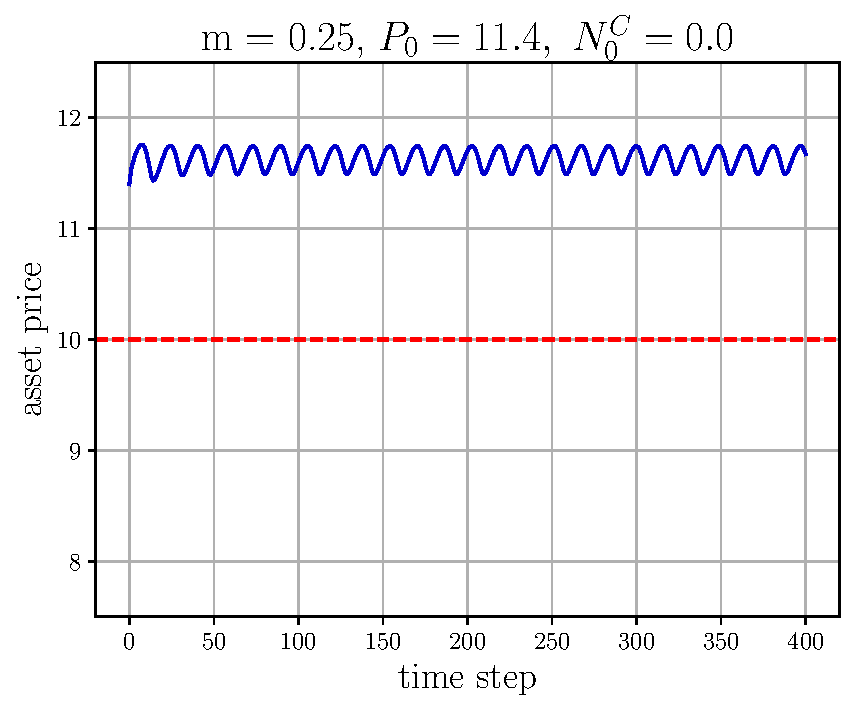
\includegraphics[width=0.4\textwidth]{../results/lean-against.pdf}\label{fig:a}}
		\hfil
		\sidesubfloat[]{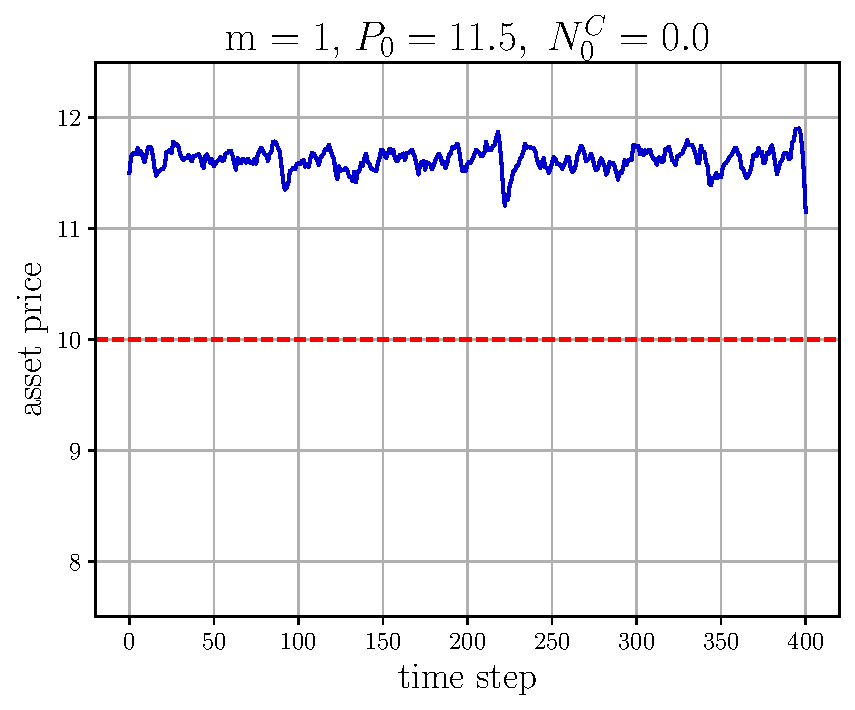
\includegraphics[width=0.4\textwidth]{../results/lean-against-stochastic.pdf}\label{fig:b}}
		
		\medskip
		\sidesubfloat[]{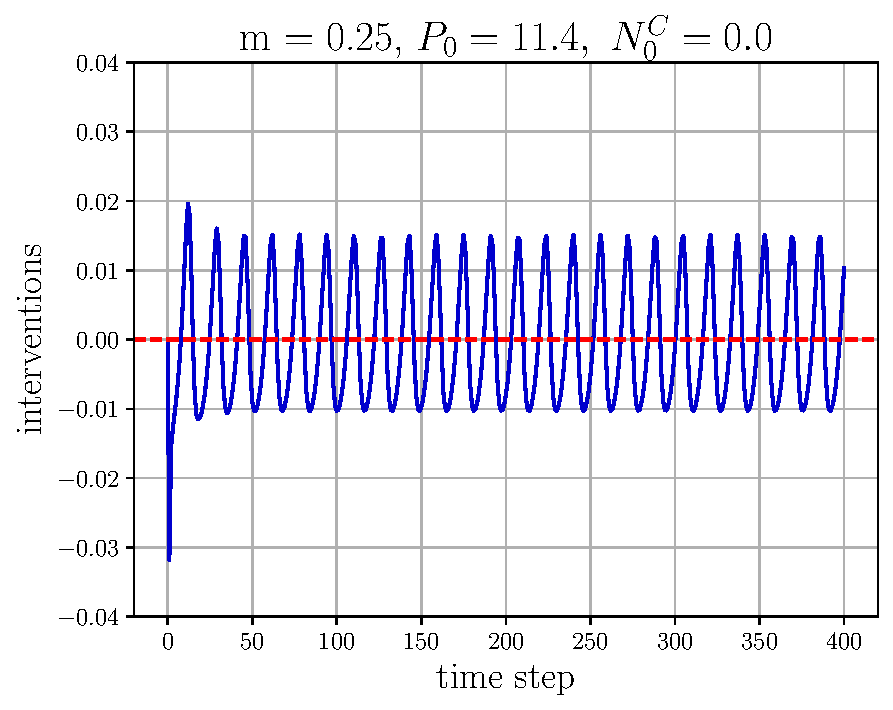
\includegraphics[width=0.4\textwidth]{../results/lean-against-intervention.pdf}\label{fig:c}}
		\hfil
		\sidesubfloat[]{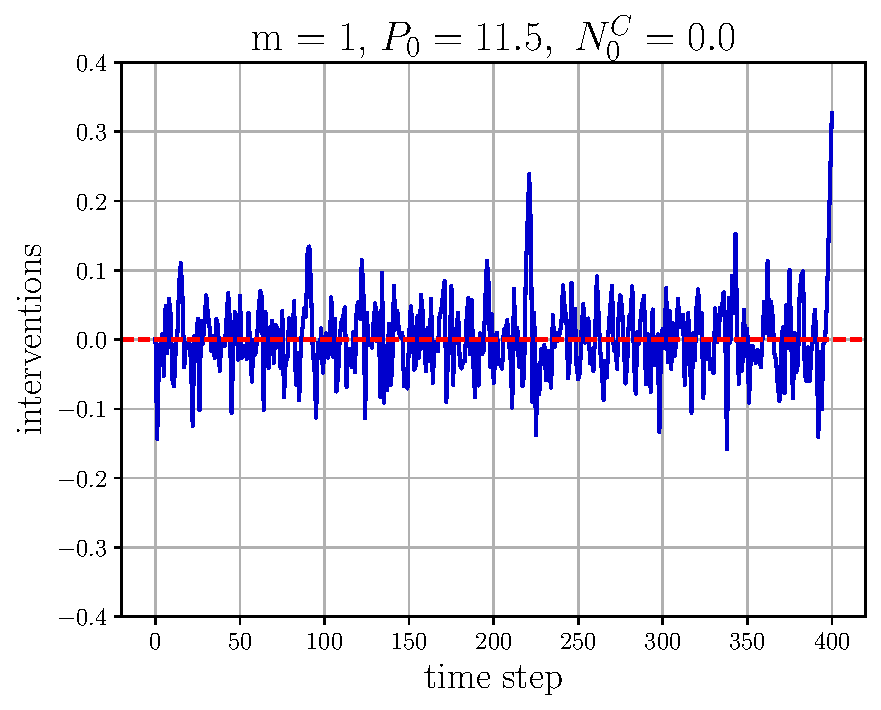
\includegraphics[width=0.4\textwidth]{../results/lean-against-intervention-stochastic.pdf}\label{fig:d}}
		
		\caption{تاثیر استراتژی فروش(خرید) در هنگام افزایش(کاهش) قیمت توسط دولت }
		\label{fig:myfigure}
	\end{figure}
در این شکل‌ها بر خلاف شکل قبل بازار تنظیم شده است. در این شکل‌ها مشاهده می‌کنیم که دولت با دخالت در بازار و حرکت دارایی‌های خود در خلاف جهت بازار باعث می‌شود تا نوسانات قیمت تا حد خوبی کاهش یابد(آ و ب). اما نتوانسته قیمت را به قیمت بنیادی کالا نزدیک کند؛ برای اینکه ببینیم آیا دولت هرگز می‌تواند با این استراتژی نه تنها نوسانات قیمت، بلکه میانگین قیمت کالا را کم کند، به سراغ نمودارهای بعدی می‌رویم.

\begin{figure}[H]
	\centering
	\sidesubfloat[]{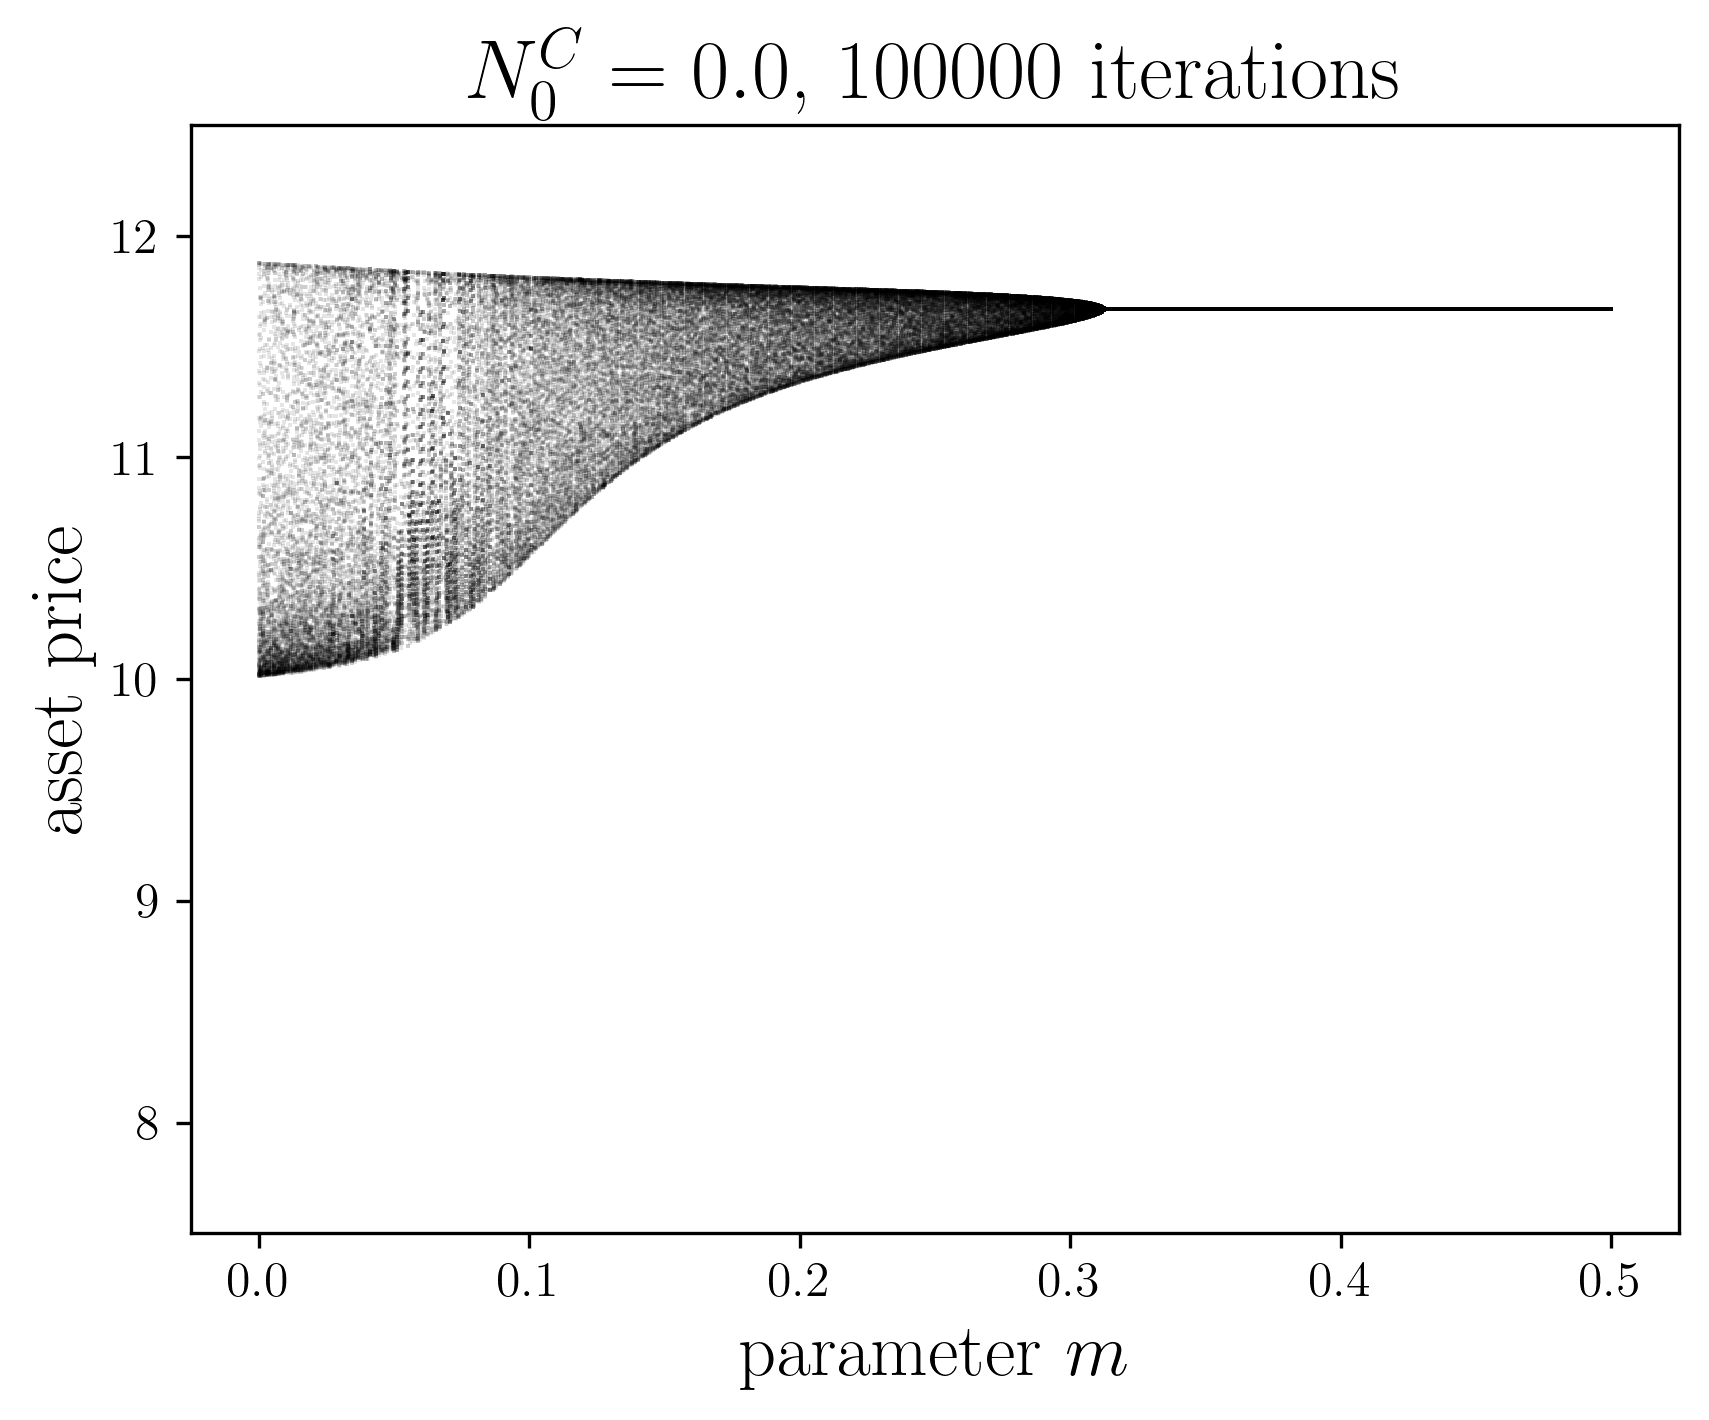
\includegraphics[width=0.4\textwidth]{../results/lean-against-bifurcation.png}\label{fig:a}}
	\hfil
	\sidesubfloat[]{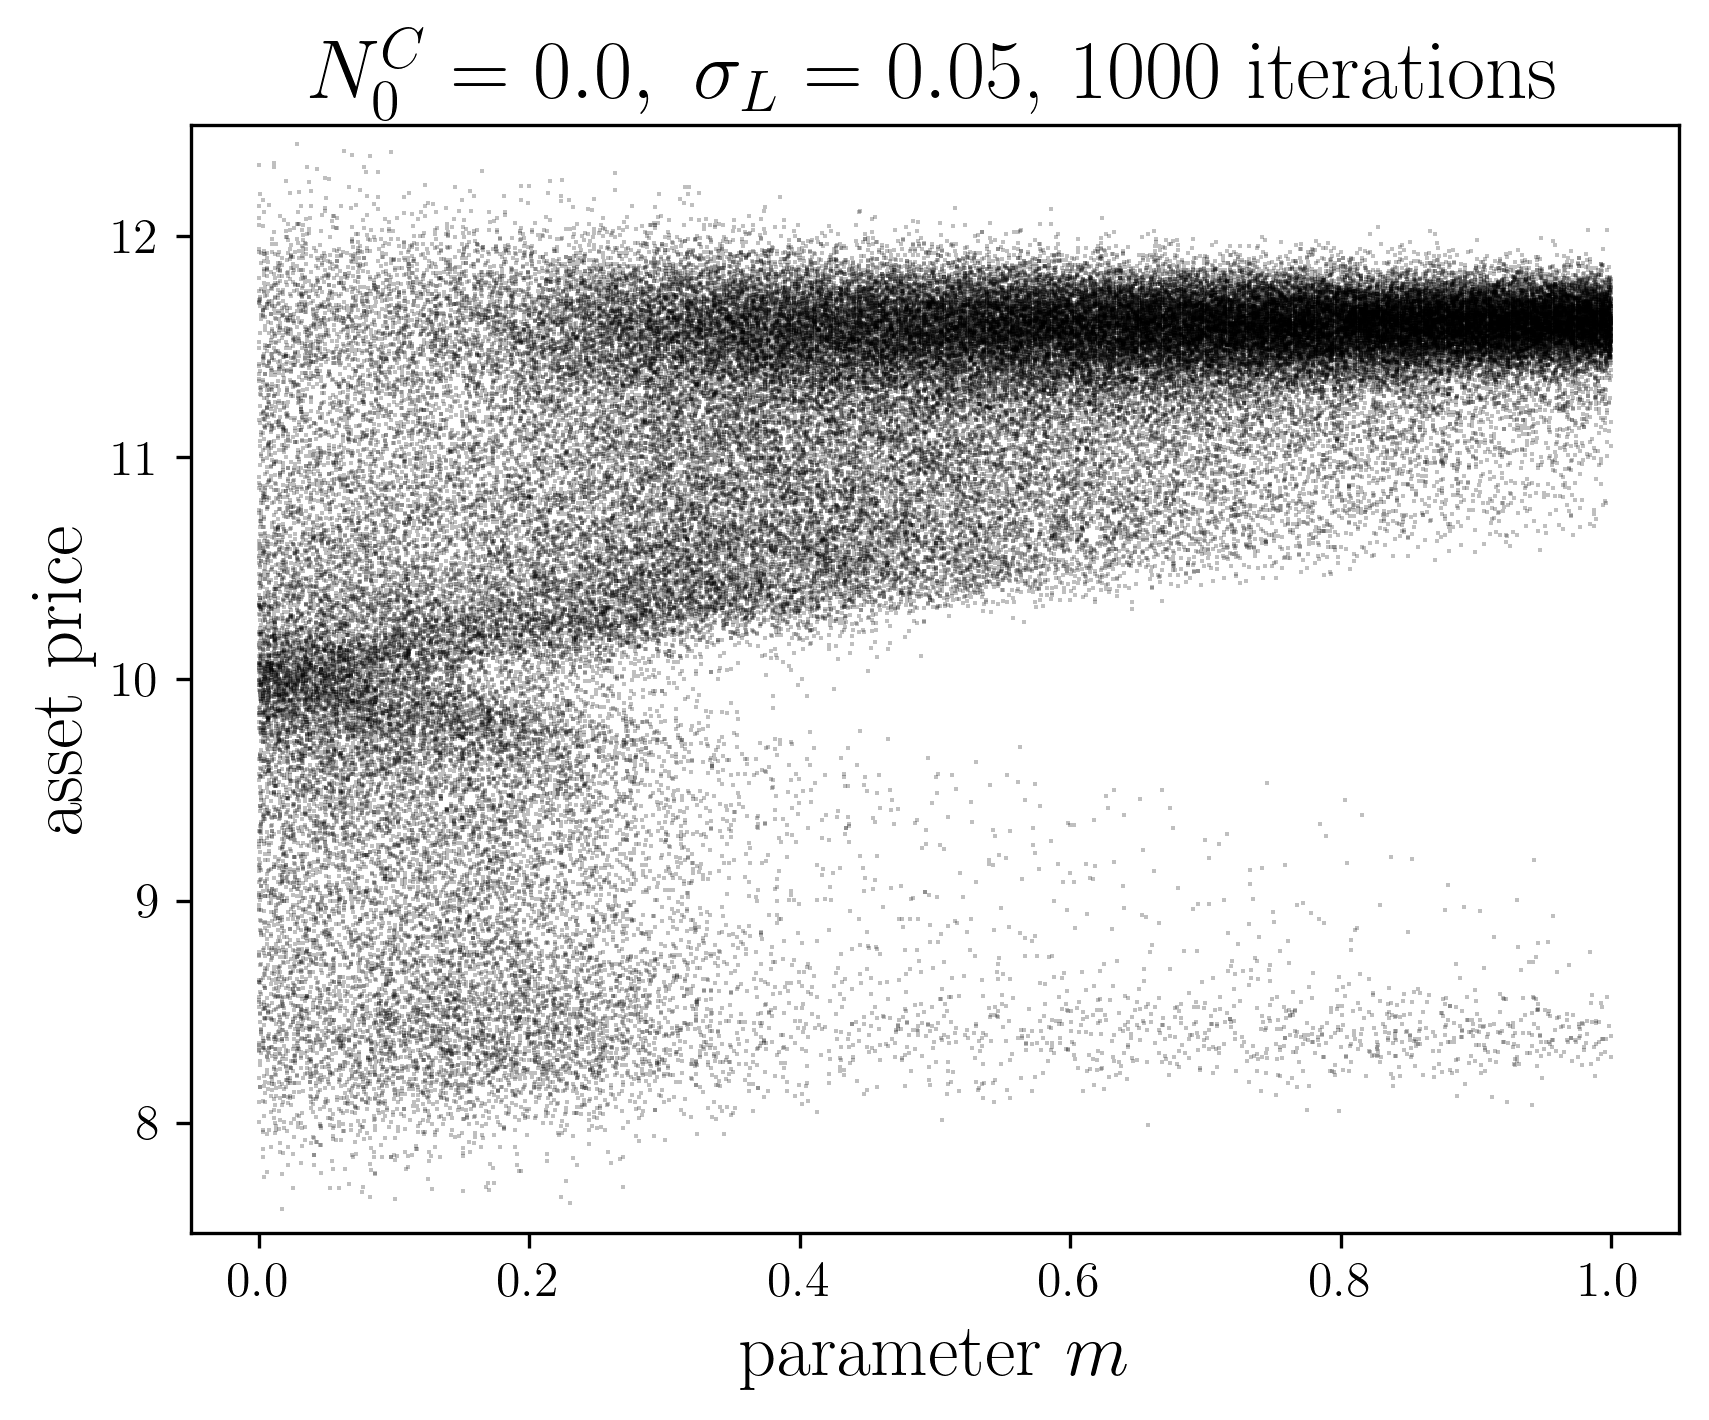
\includegraphics[width=0.4\textwidth]{../results/lean-against-bifurcation-stochastic.png}\label{fig:b}}
	
	\medskip
	\sidesubfloat[]{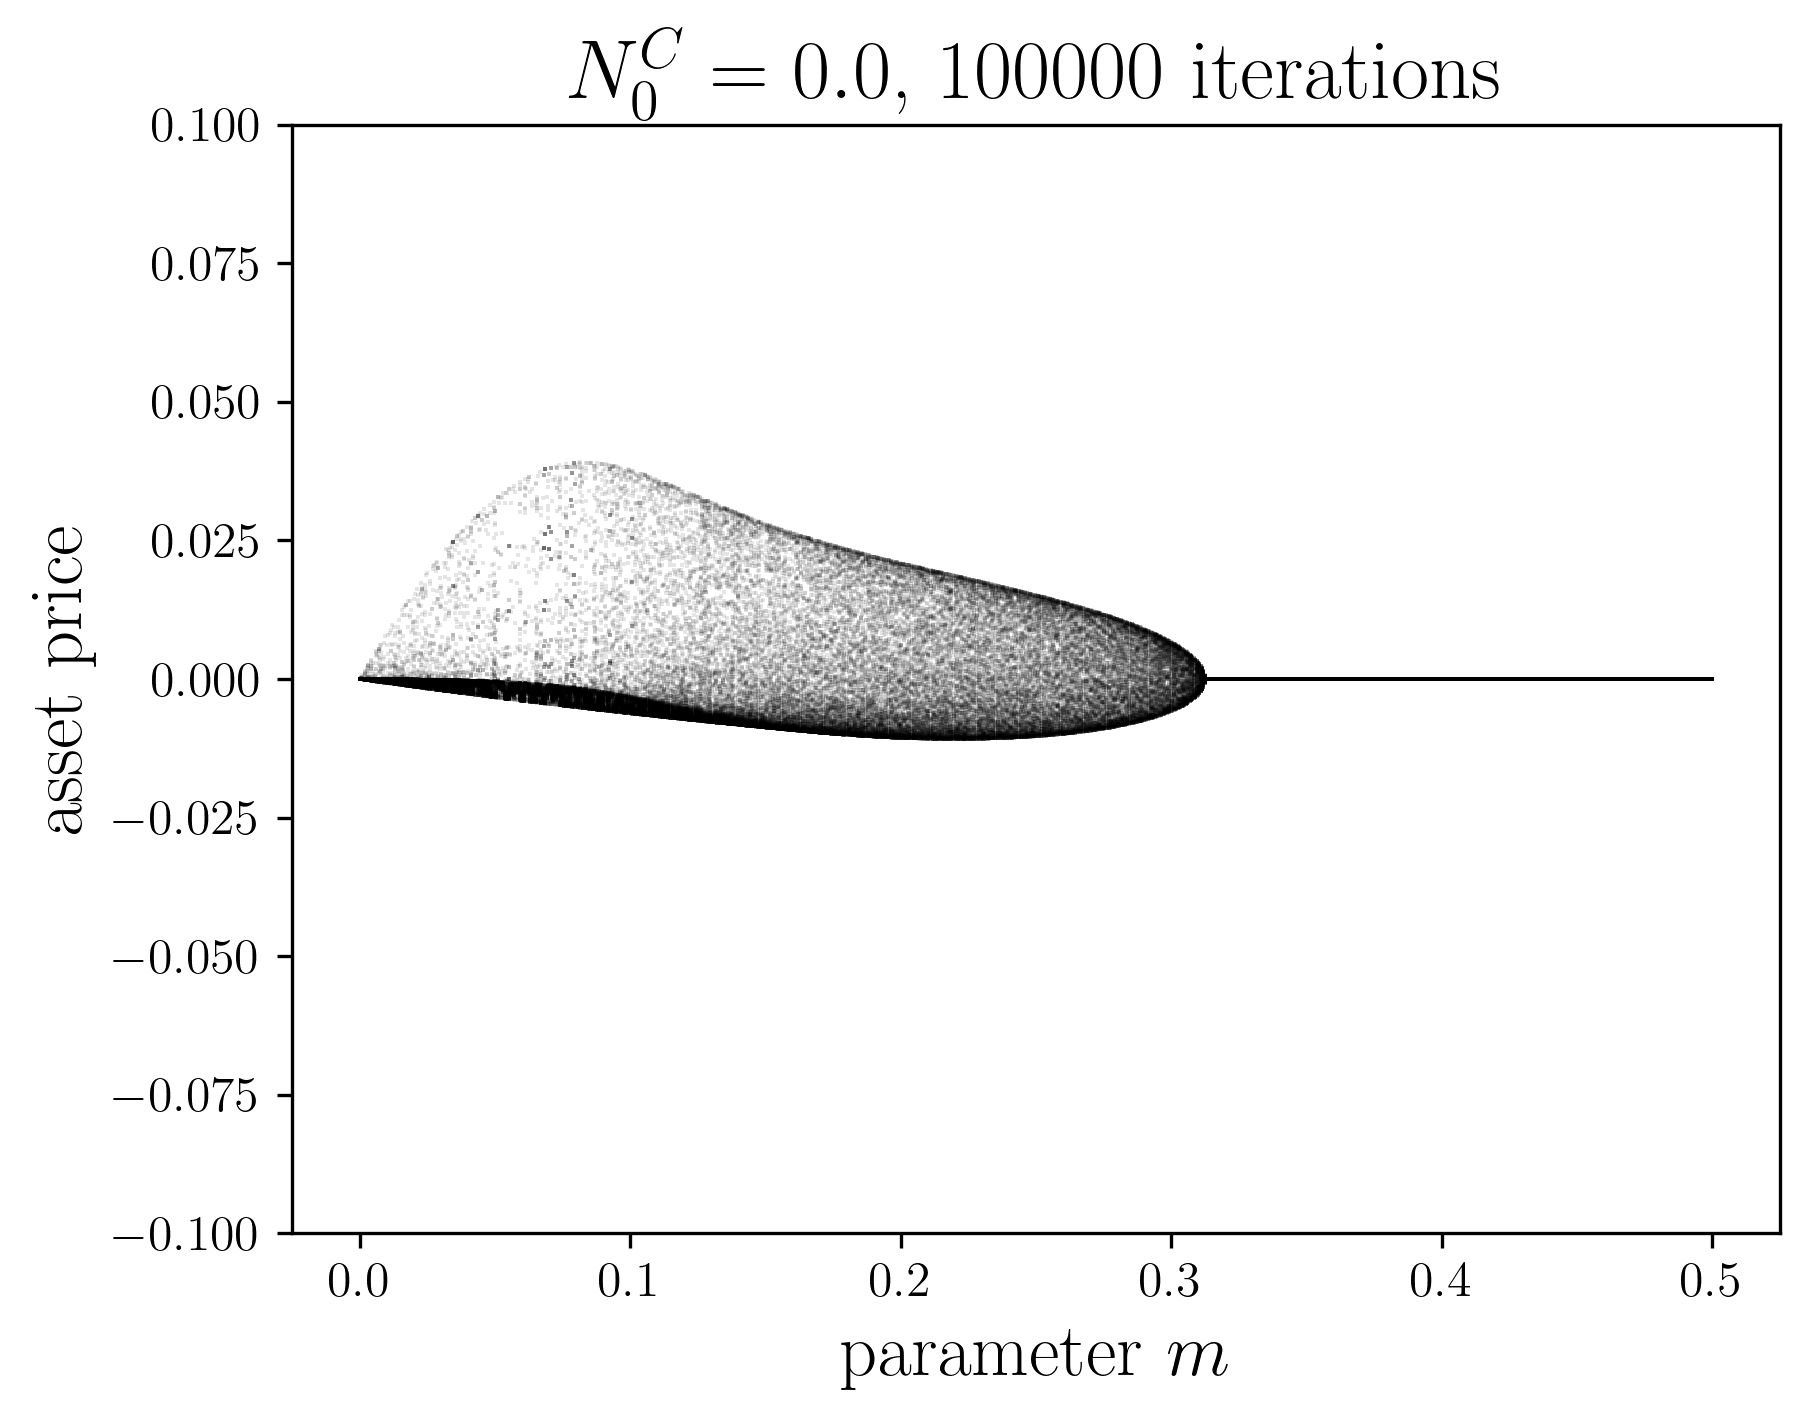
\includegraphics[width=0.4\textwidth]{../results/lean-against-bifurcation-intervention.png}\label{fig:c}}
	\hfil
	\sidesubfloat[]{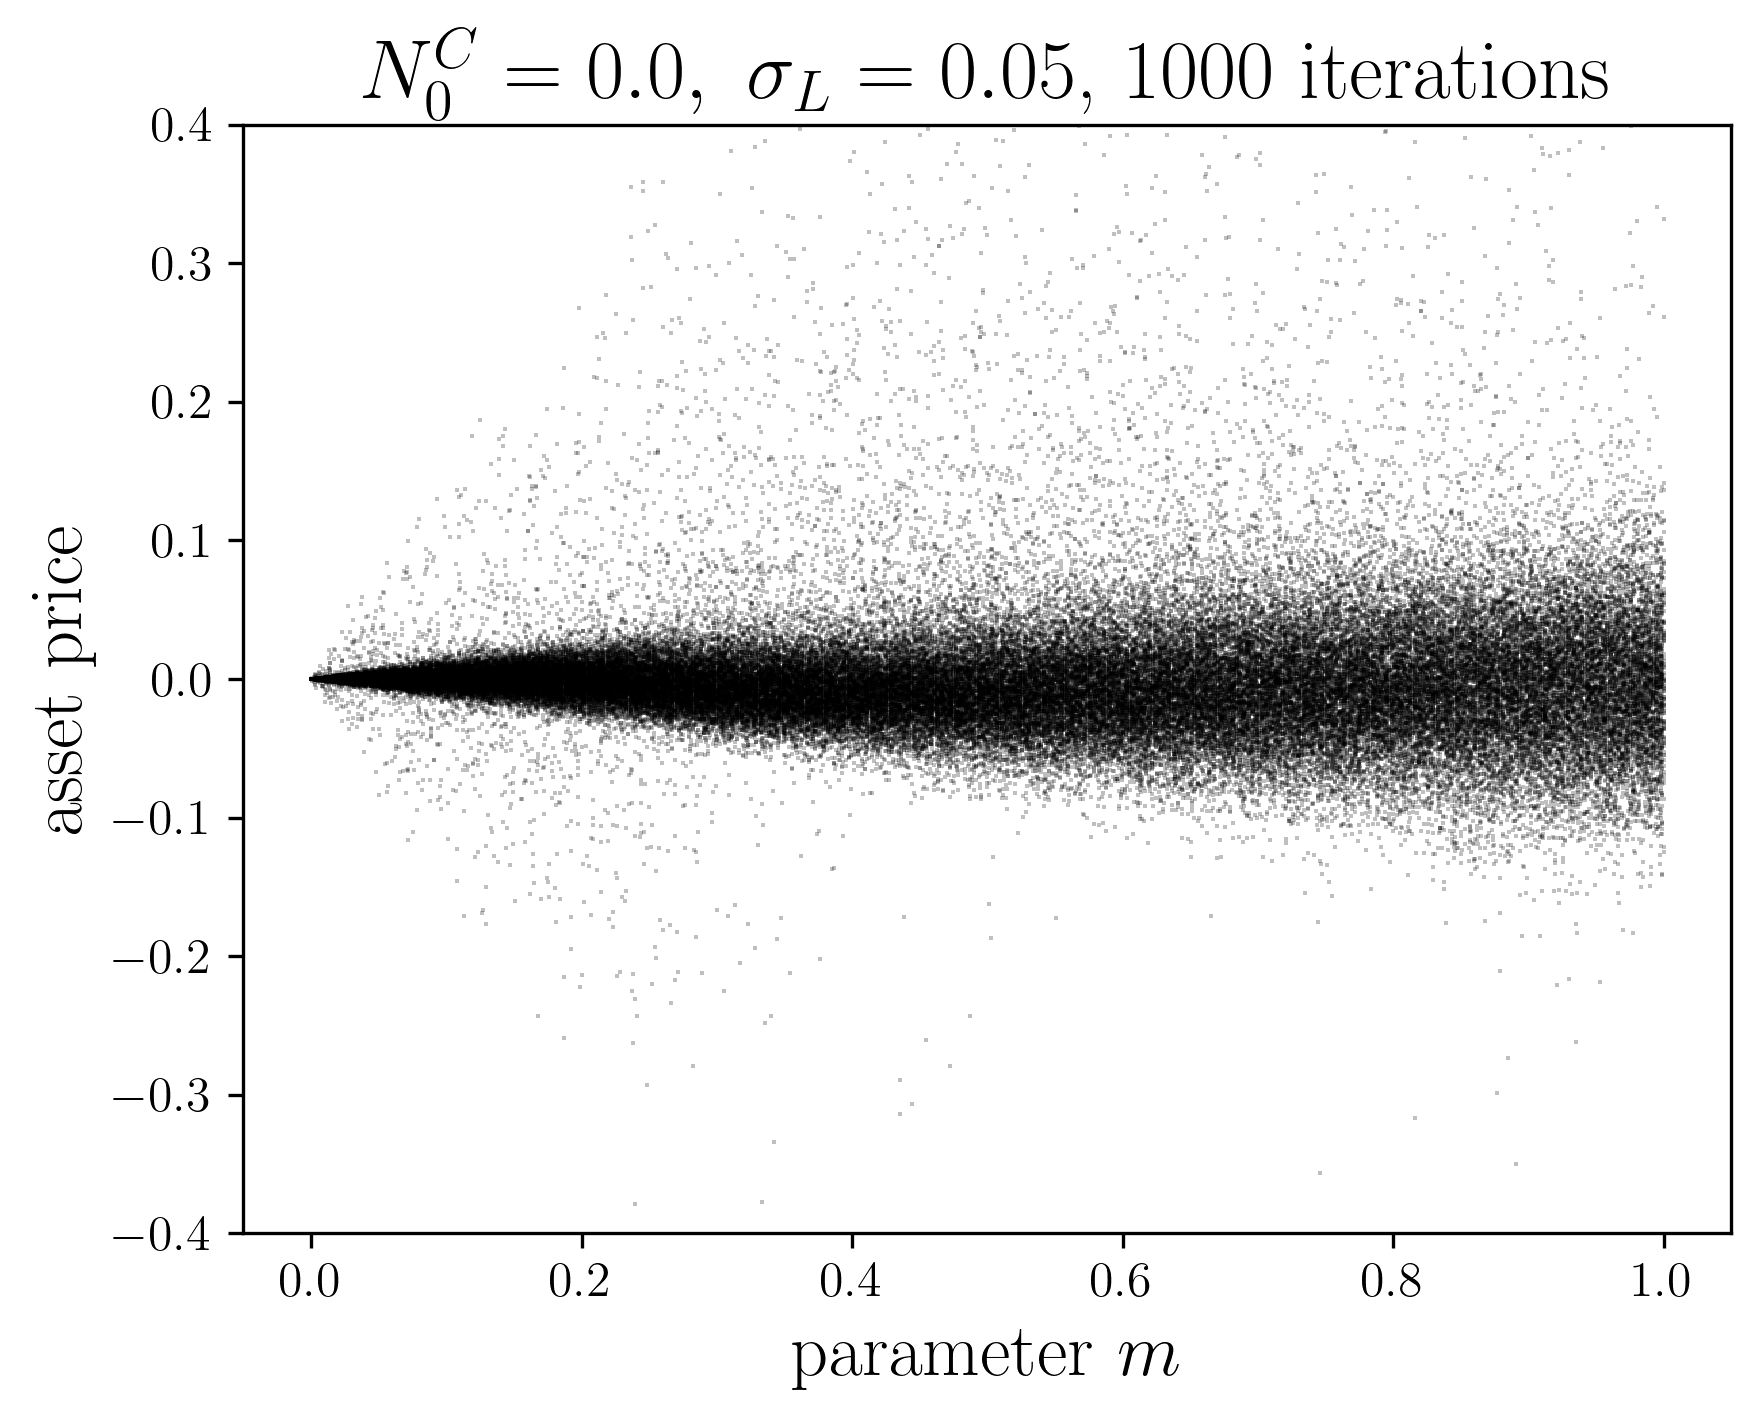
\includegraphics[width=0.4\textwidth]{../results/lean-against-bifurcation-stochastic-intervention.png}\label{fig:d}}
	
	\caption{تغییر پایداری قیمت‌ها تحت تاثیر تنظیم بازار }
	\label{fig:myfigure}
\end{figure}
	در این جا پایداری قیمت‌ها با احتساب تغییر دخالت دولت در بازار با استراتژی اول مشاهده می‌شود. حتی در حالتی که عدم قطعیت نداریم، برای آن که بازار از حالت غیر پایدار خارج شود باید پارامتر $m$ را به حدود $0.3$ برسانیم. و حتی پس آنکه این پارامتر را به $0.5$ رساندیم میبینیم نوسانات بازار کاهش یافته اما قیمت همچنان بالا تر از قیمت بنیادی است. دوباره با اعمال کمی عدم قطعیت به سیستم (ب و د) می‌بینیم که باز خم‌های پایدار پهن می‌شوند و به طور مثال در $m=0.3$ که حالت بدون نوفه یک نقطه ثابت پایدار داشت حالا کاملا ناپایدار شده است.
	
	
	
	\begin{figure}[H]
	\centering
	\sidesubfloat[]{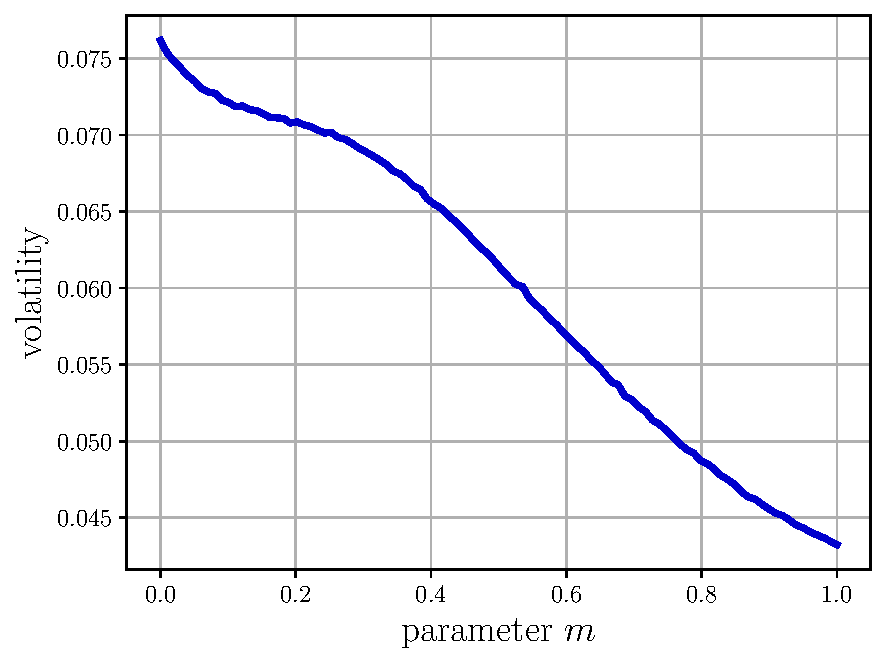
\includegraphics[width=0.4\textwidth]{../results/lean-against-volatility.pdf}\label{fig:a}}
	\hfil
	\sidesubfloat[]{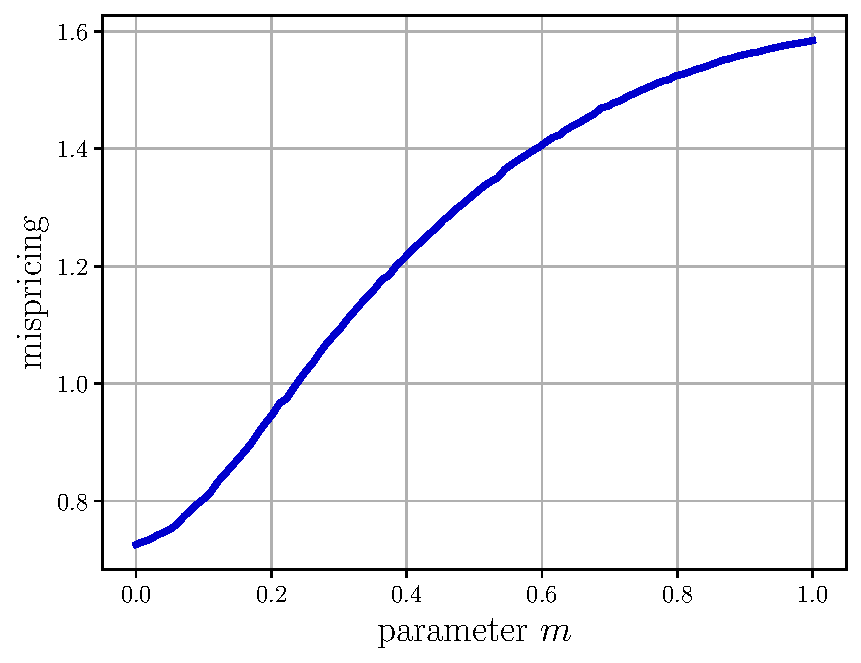
\includegraphics[width=0.4\textwidth]{../results/lean-against-mispricing.pdf}\label{fig:b}}
	
	\medskip
	\sidesubfloat[]{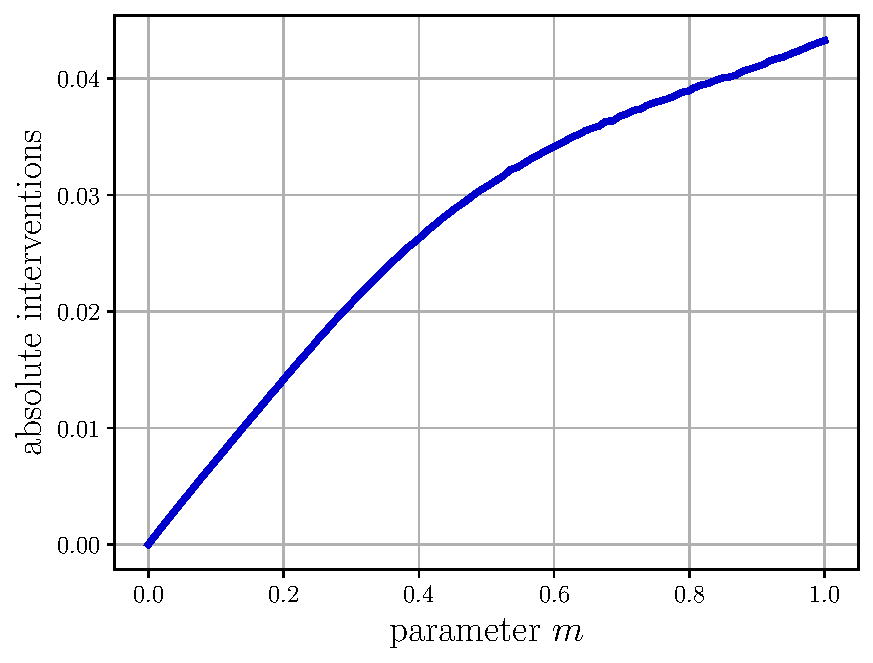
\includegraphics[width=0.4\textwidth]{../results/lean-against-absint.pdf}\label{fig:c}}
	\hfil
	\sidesubfloat[]{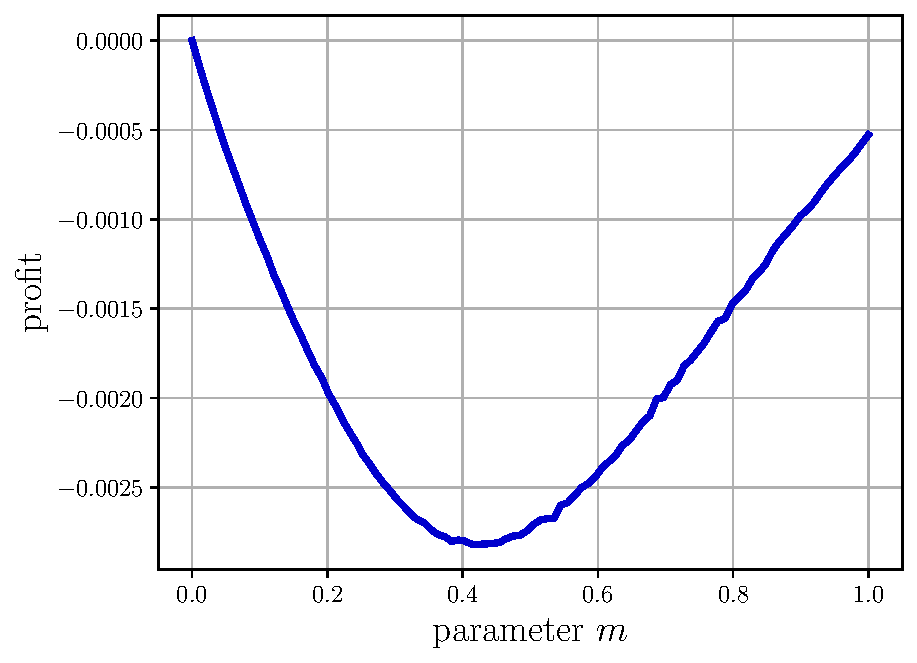
\includegraphics[width=0.4\textwidth]{../results/lean-against-profit.pdf}\label{fig:d}}
	
	\medskip
	\sidesubfloat[]{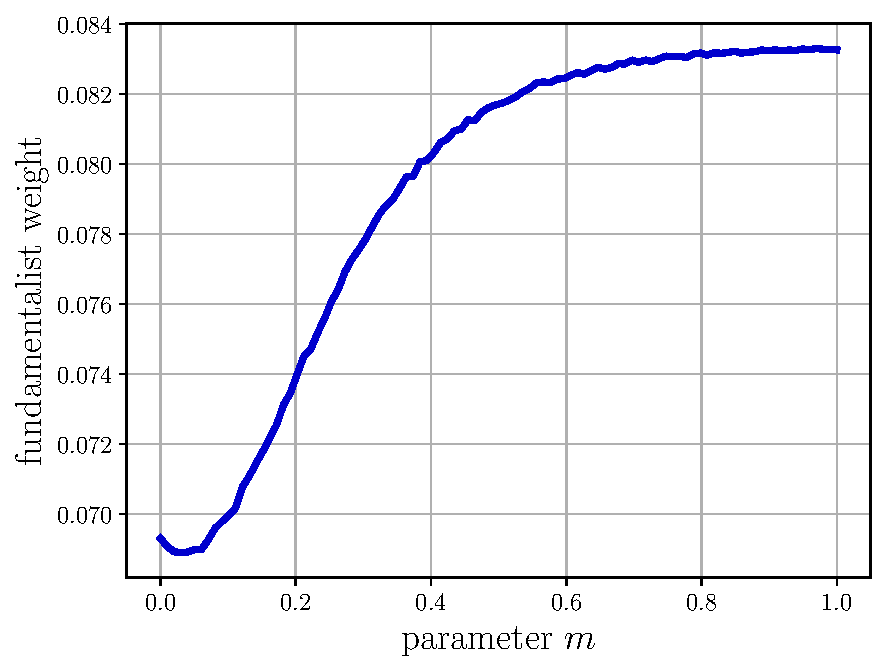
\includegraphics[width=0.4\textwidth]{../results/lean-against-fundweight.pdf}\label{fig:e}}
	\hfil
	\sidesubfloat[]{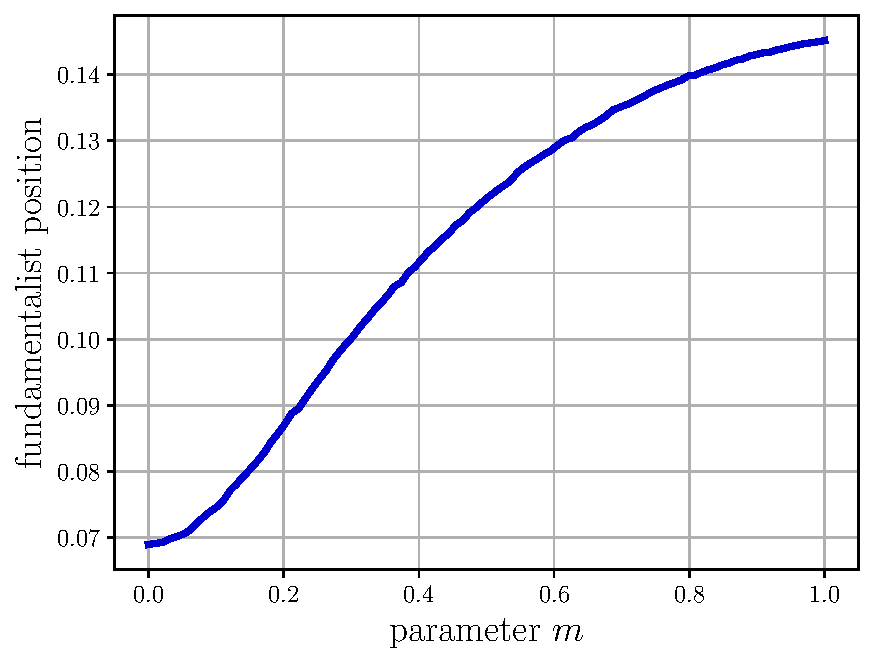
\includegraphics[width=0.4\textwidth]{../results/lean-against-fundpos.pdf}\label{fig:f}}
	\caption{تاثیر دخالت دولت در بازار}
	\label{fig:myfigure}
\end{figure}
در این شش نمودار به اندازه گیری شش سنجه می‌پردازیم تا ببینیم سیاست دولت در راستای تنظیم بازار چقدر مفید بوده است. ابتدا تاثیر آن بر تلاطم\footnote{\lr{volatility}} (میانگین اندازه تغییرات) قیمت در بازه زمانی اعمال دخالت(آ)، سپس بر قیمت گذاری نادرست (میانگین فاصله‌ی قیمت بازار و قیمت بنیادی. شکل ب)، میزان دخالت دولت در بازار (مجموع مقدار کالایی که در بازار مبادله کرده. شکل ج)، سود دولت از این مبادلات (د)، میانگین کسر بنیادگرای\footnote{\lr{$\bar{N}_F$}} جمعیت(ه) و در نهایت میزان مبادلات بنیادگرایان(و). با این که دولت با افزایش دخالت در بازار می‌تواند تطاطم بازار را کاهش دهد همزمان قیمت را افزایش می‌دهد که به ضرر بازار است(آ و ب). و همچنین چون دولت کاملا بر خلاف بازار عمل می‌کند سودش منفی است. به همین علت همیشه در حال ضرر است. همچنین به طور بسیار جزئی کسر بینادگرایان و میزان مبادلات آن‌ها را افزایش می‌د‌هد؛ جزئی به این دلیل که وقتی پارامتر $m$ را ده برابر می‌کنیم، کسر بنیادگرایان دو برابر و مبادلات آن‌ها تنها ۱۸ درصد رشد می‌کند.

\begin{figure}[H]
	\centering
	\sidesubfloat[]{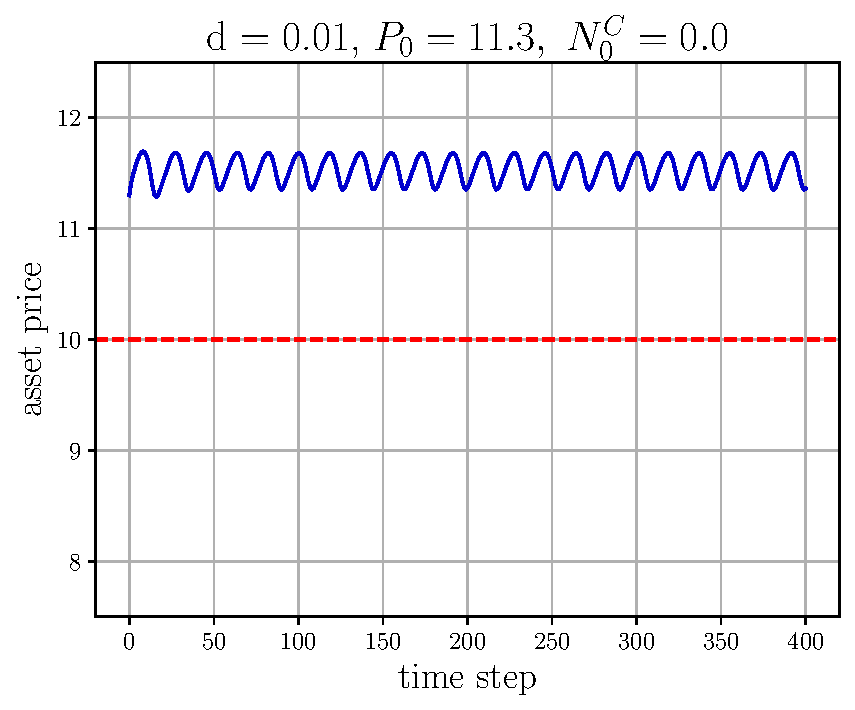
\includegraphics[width=0.4\textwidth]{../results/target-fundamental.pdf}\label{fig:a}}
	\hfil
	\sidesubfloat[]{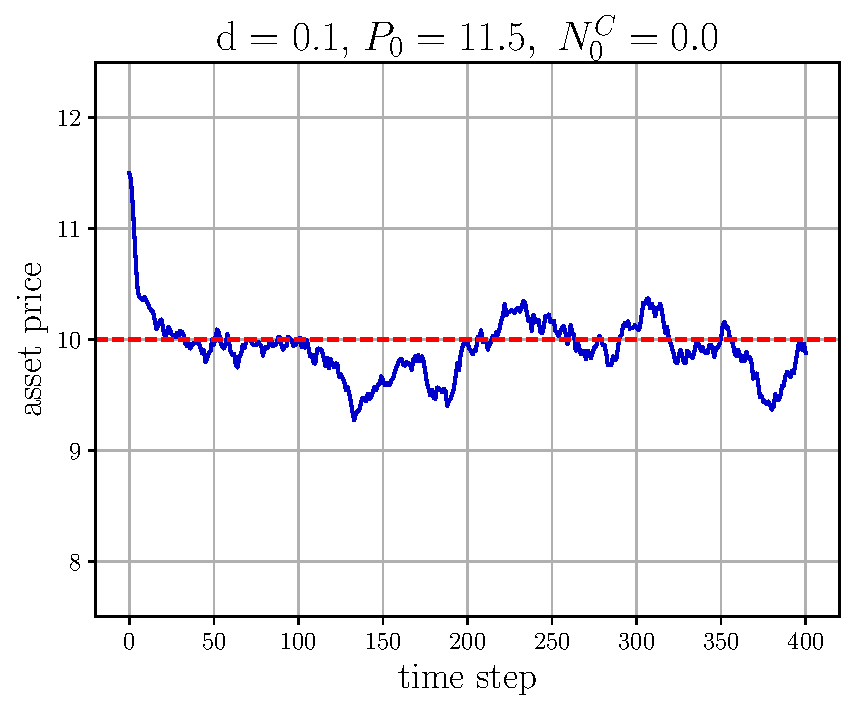
\includegraphics[width=0.4\textwidth]{../results/target-fundamental-stochastic.pdf}\label{fig:b}}
	
	\medskip
	\sidesubfloat[]{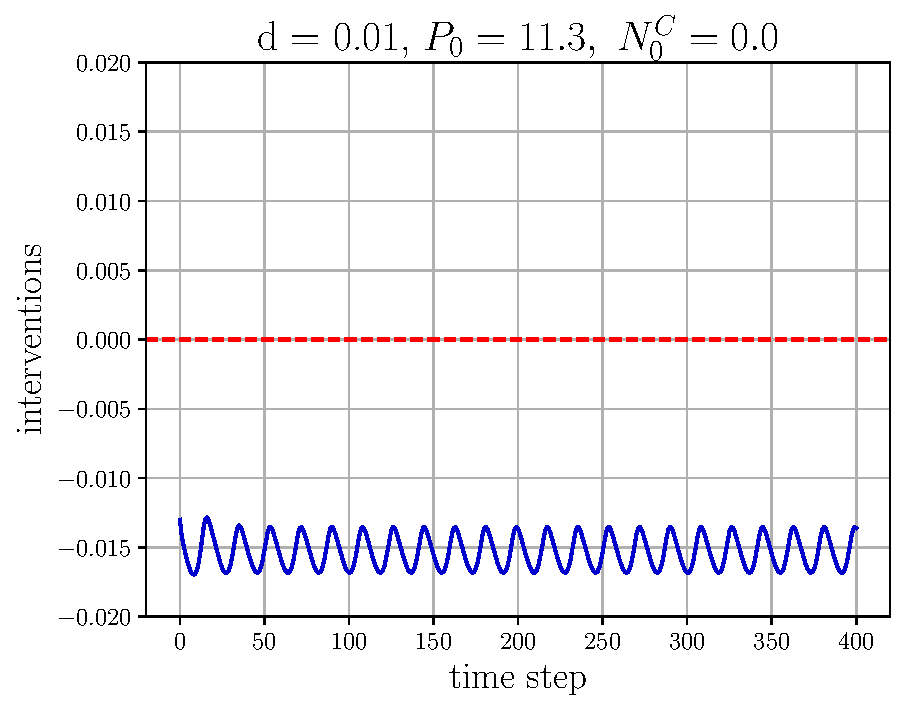
\includegraphics[width=0.4\textwidth]{../results/target-fundamental-intervention.pdf}\label{fig:c}}
	\hfil
	\sidesubfloat[]{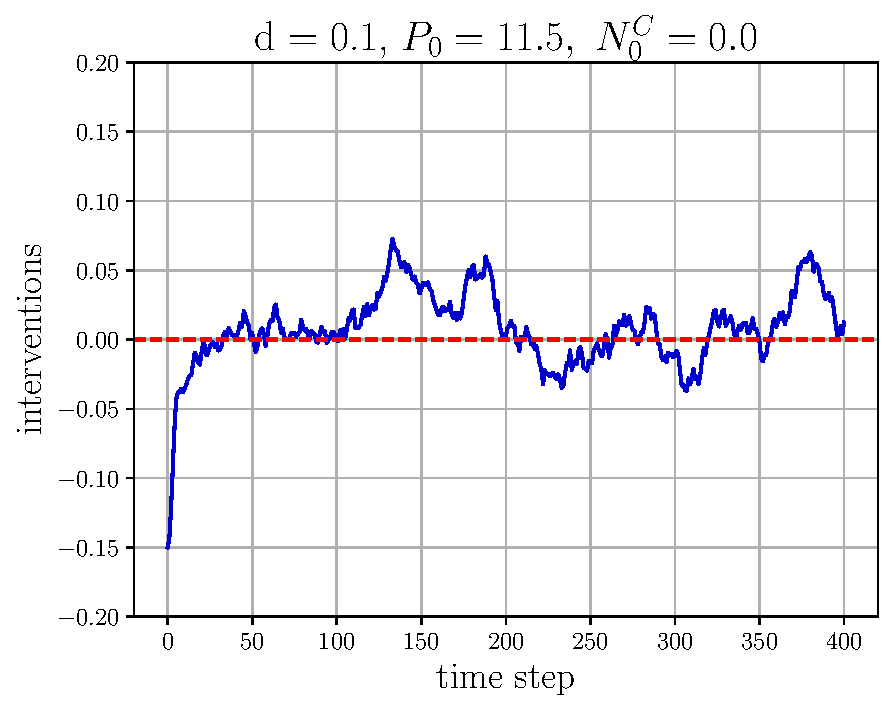
\includegraphics[width=0.4\textwidth]{../results/target-fundamental-intervention-stochastic.pdf}\label{fig:d}}
	
	\caption{تاثیر استراتژی هدایت قیمت دولت}
	\label{fig:myfigure}
\end{figure}
به طور مشابه با استراتژی قبلی مشکلات مشترک بین دو استراتژی وجود دارد اما نکته قابل توجه این است که پارامتر کنترل ما در این قسمت $0.04$ برابر پارامتر کنترل ما در قسمت قبل است. به همین دلیل احتمال کنترل پذیری سیستم توسط این پارامتر آسان‌تر انجام می‌شود.

\begin{figure}[H]
	\centering
	\sidesubfloat[]{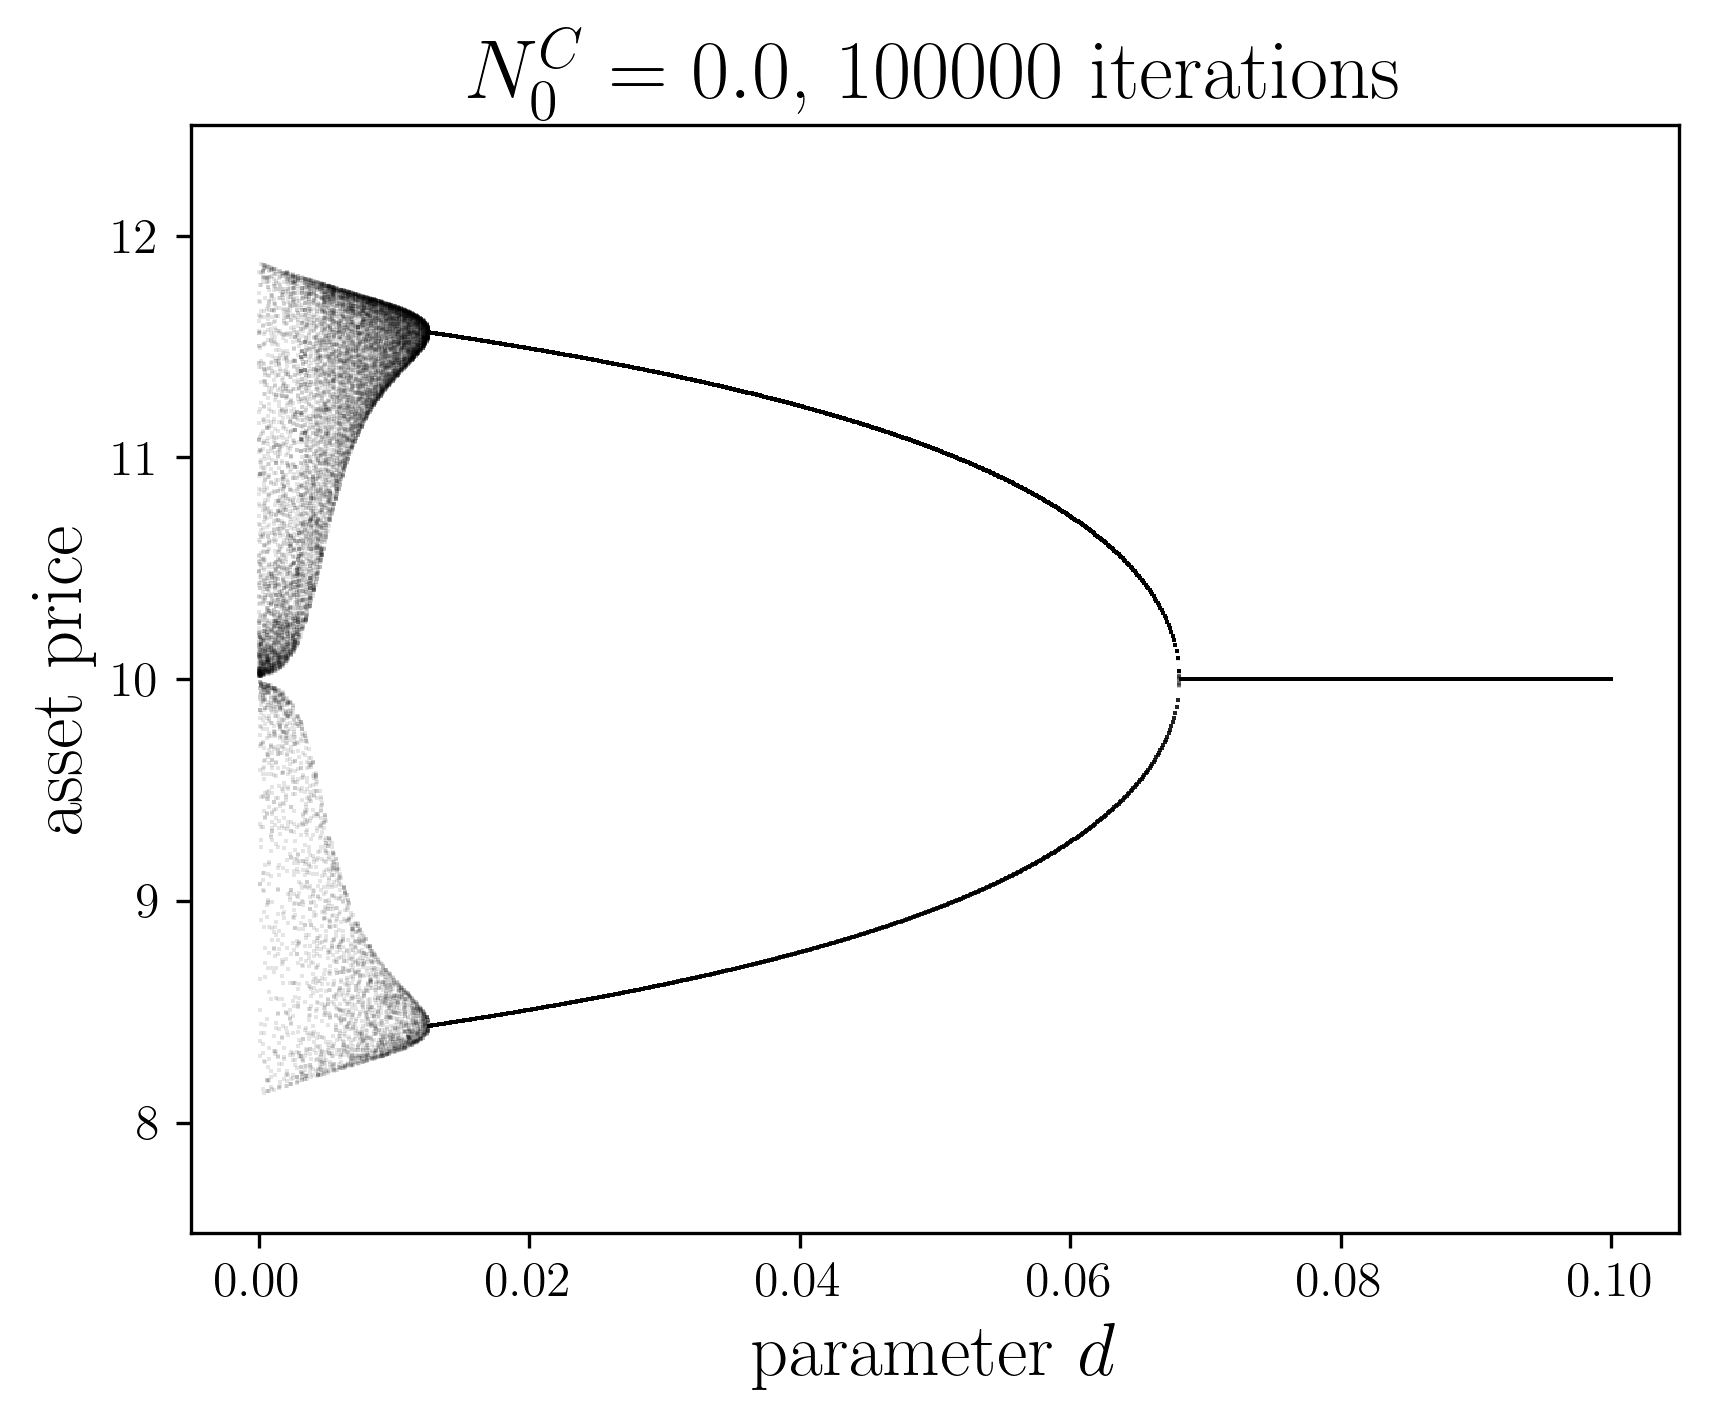
\includegraphics[width=0.4\textwidth]{target-fundamental-bifurcation.png}\label{fig:a}}
	\hfil
	\sidesubfloat[]{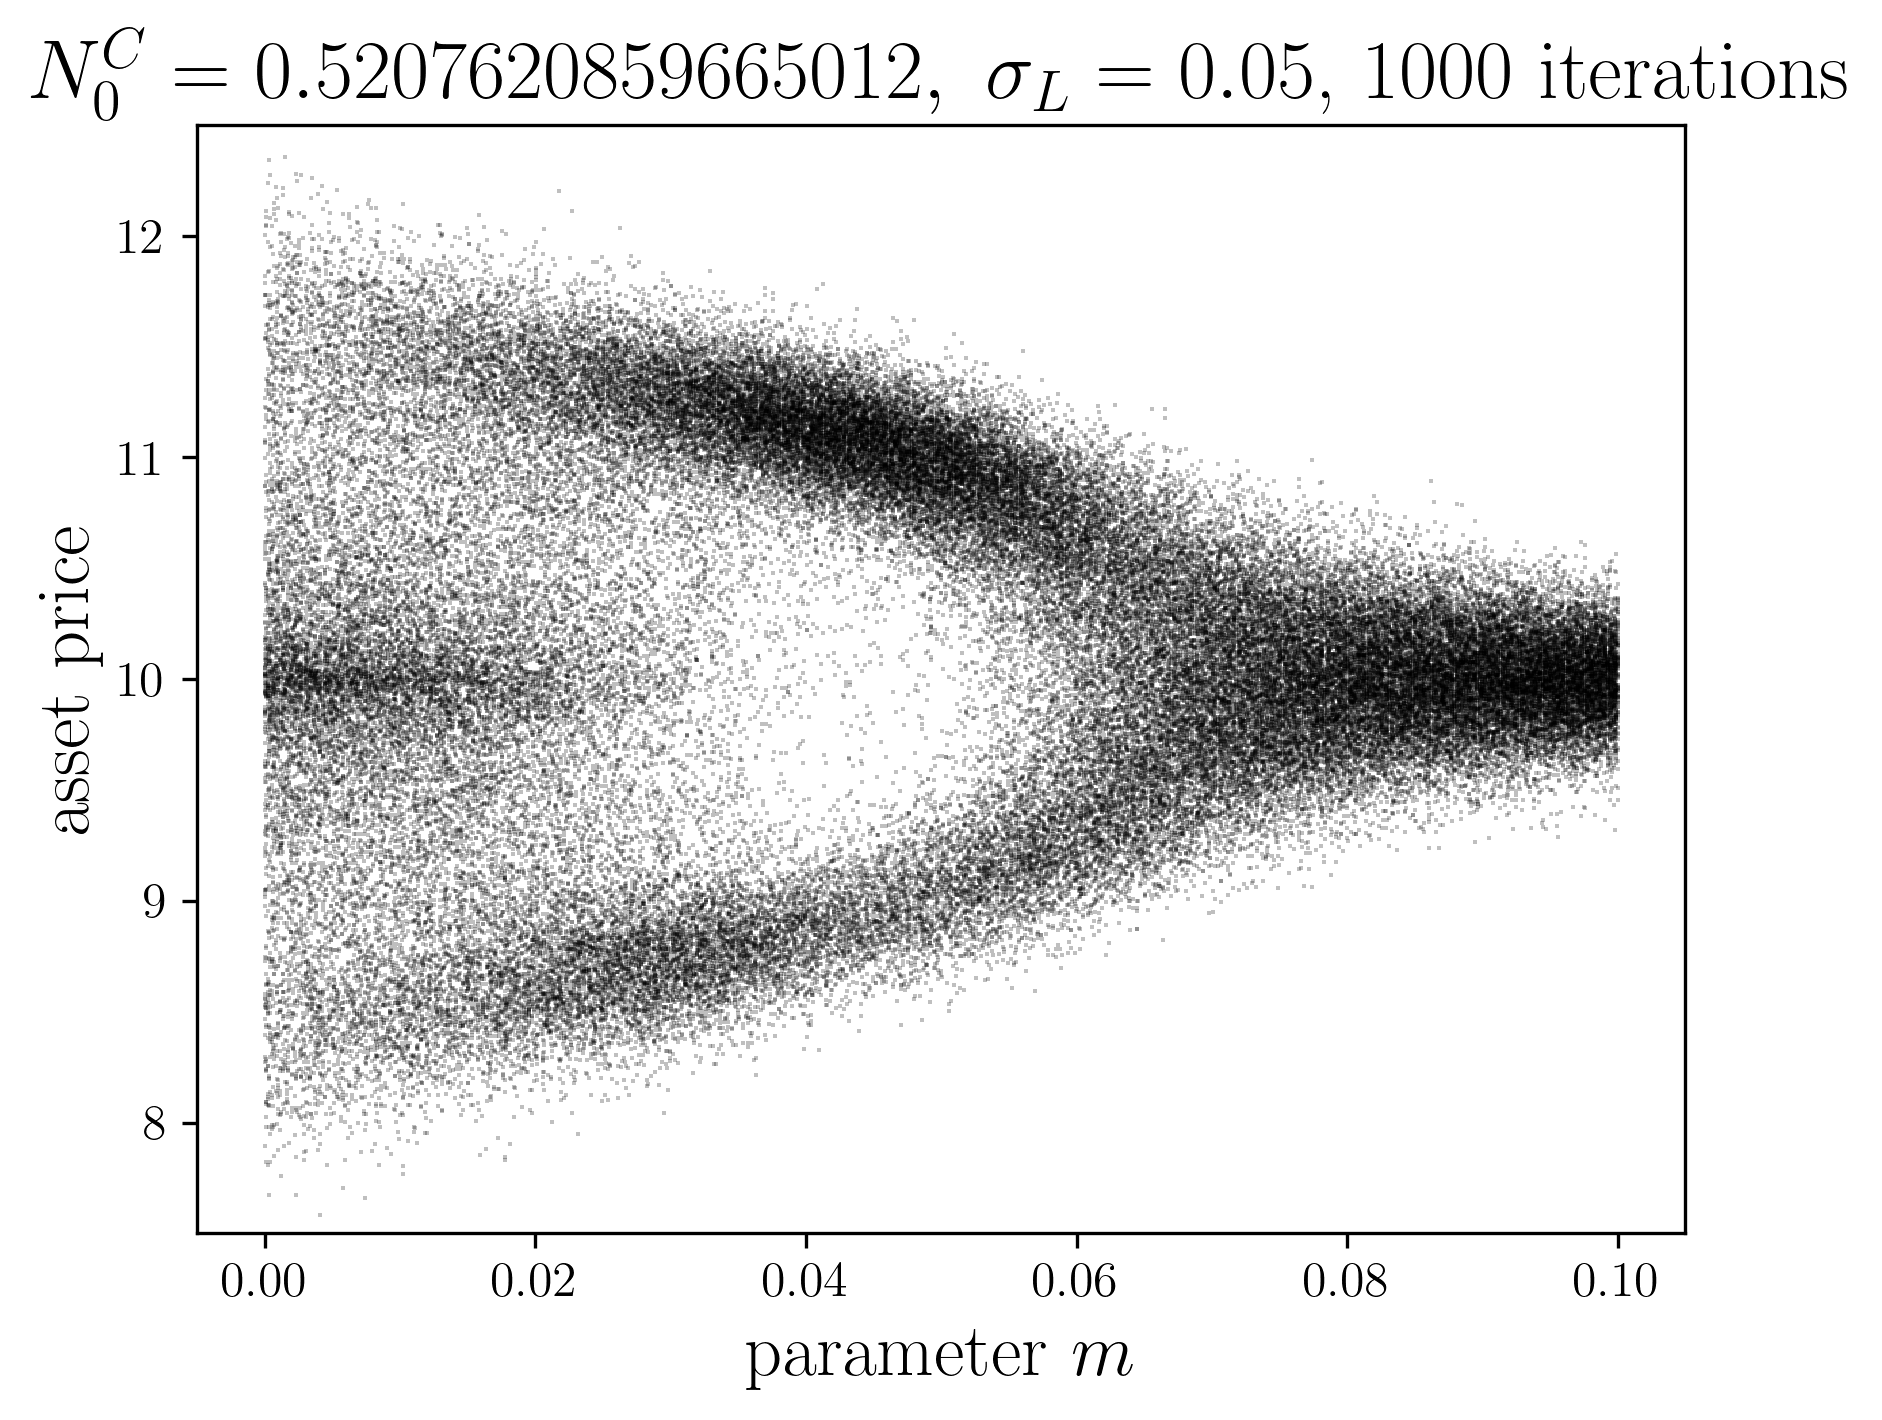
\includegraphics[width=0.4\textwidth]{target-fundamental-bifurcation-stochastic.png}\label{fig:b}}
	
	\medskip
	\sidesubfloat[]{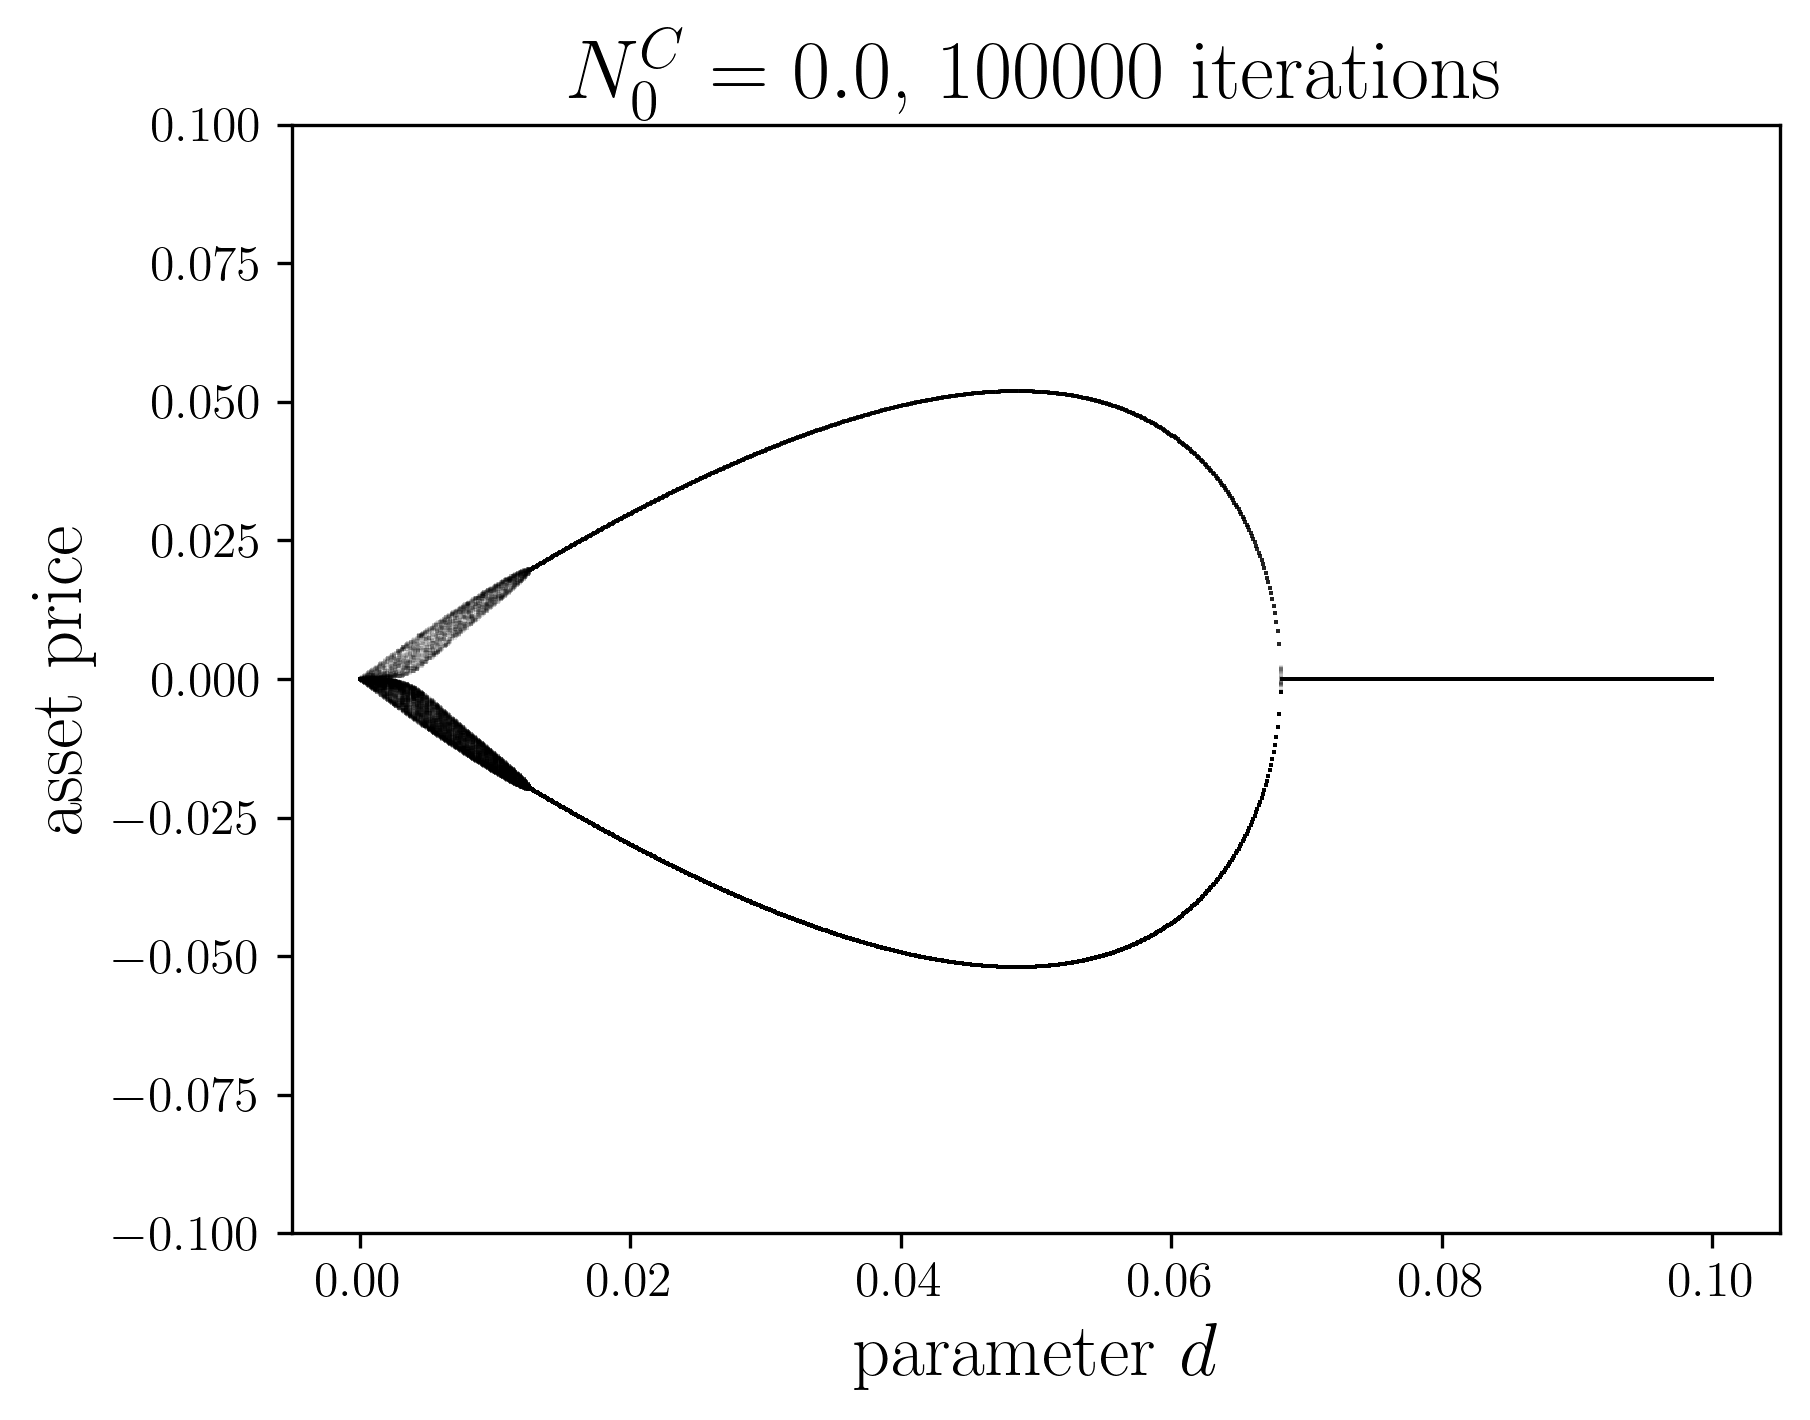
\includegraphics[width=0.4\textwidth]{target-fundamental-bifurcation-intervention.png}\label{fig:c}}
	\hfil
	\sidesubfloat[]{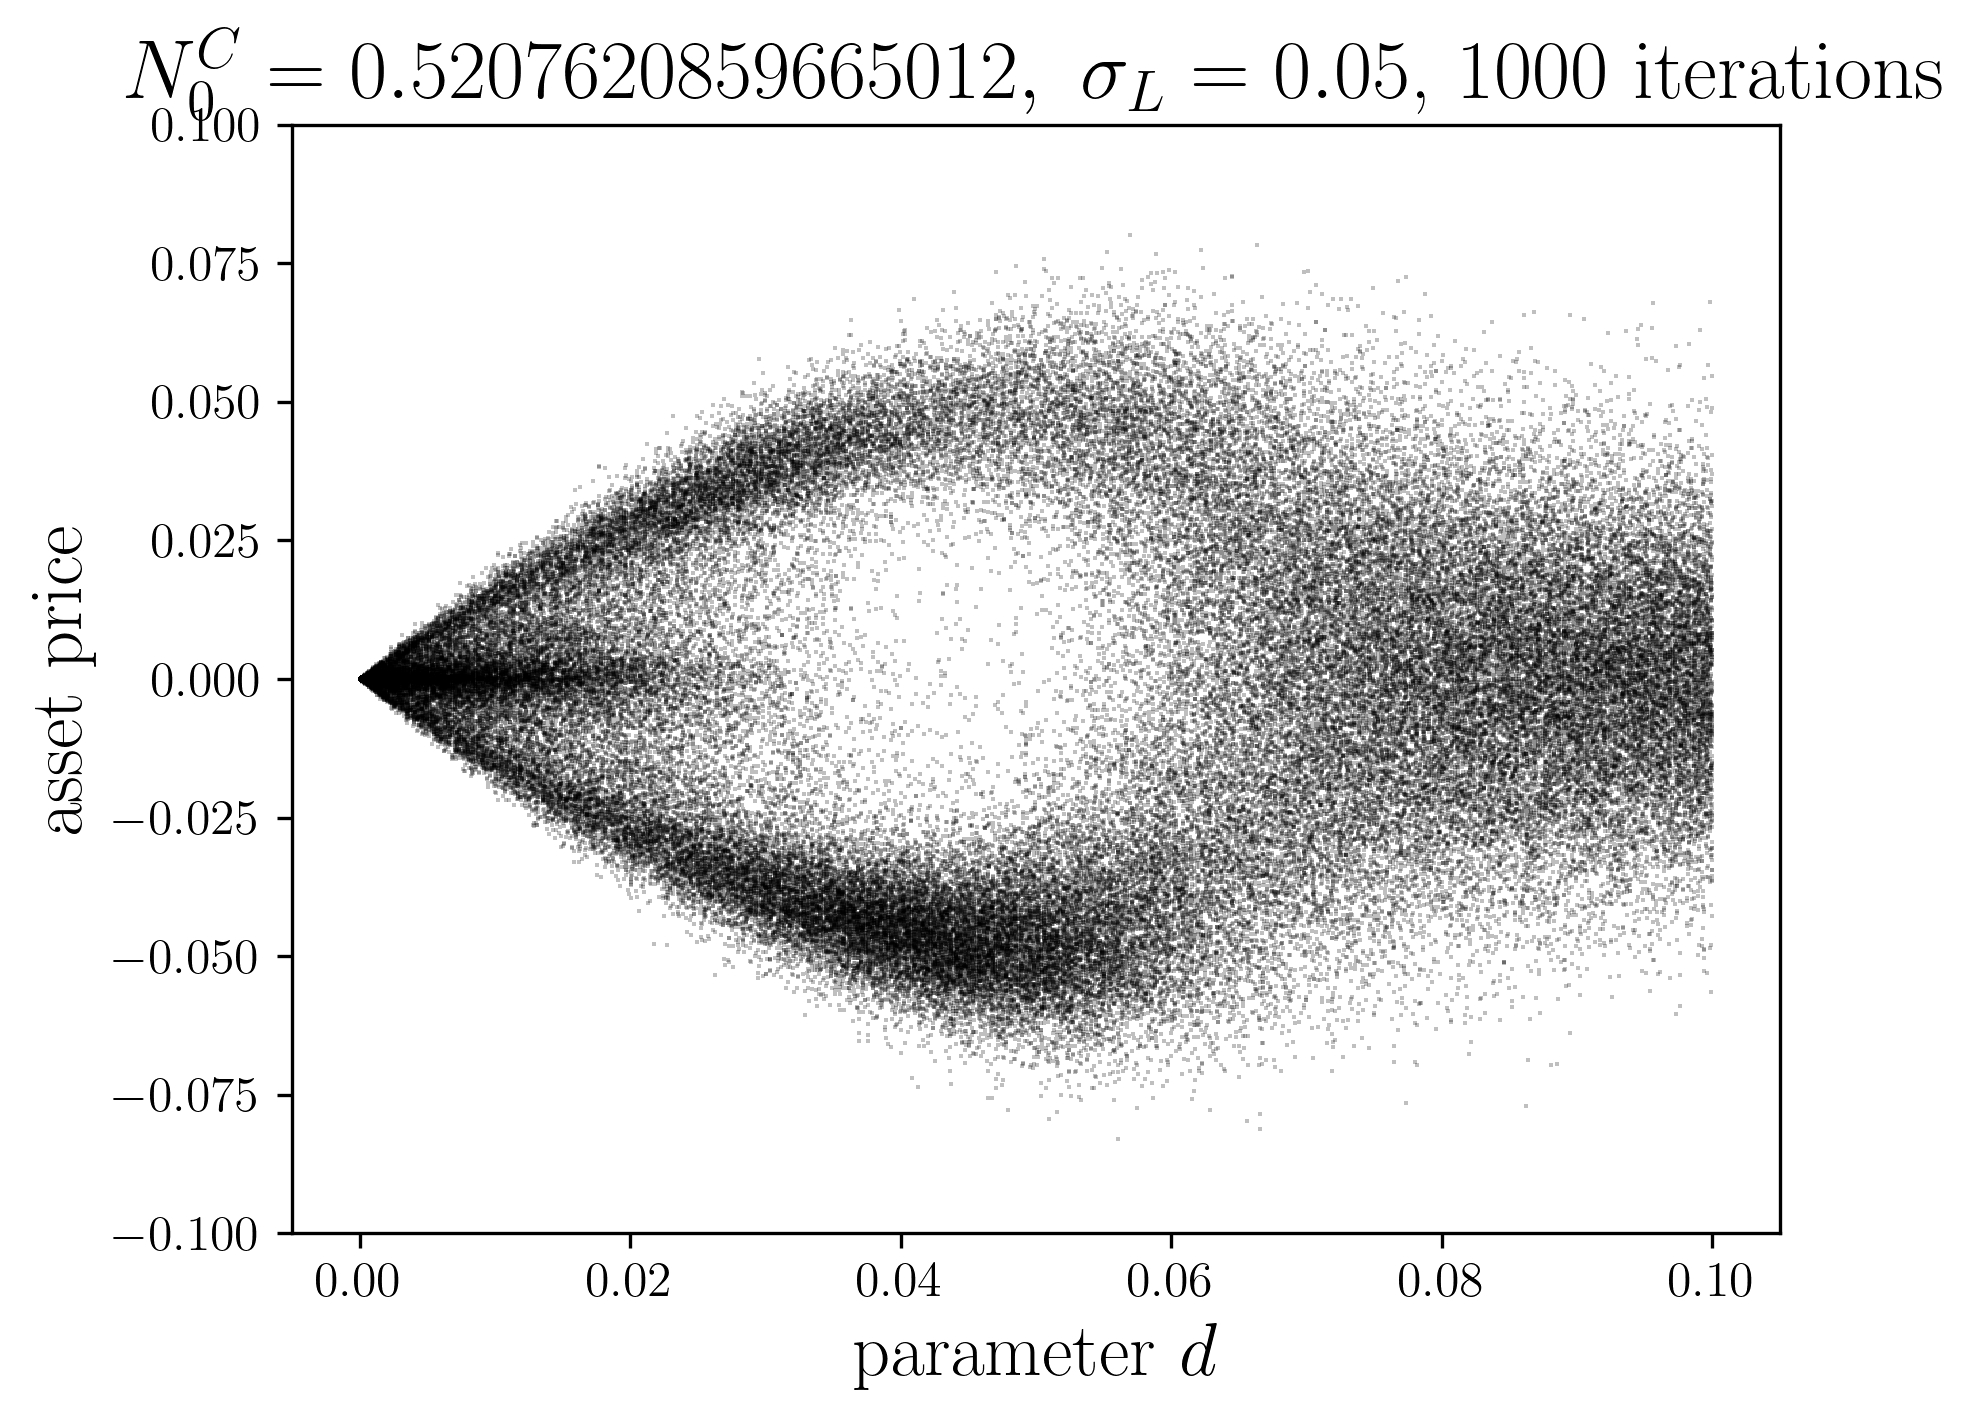
\includegraphics[width=0.4\textwidth]{target-fundamental-bifurcation-stochastic-intervention.png}\label{fig:d}}
	
	\caption{تاثیر استراتژی هدایت قیمت روی تعادل بازار}
	\label{fig:myfigure}
\end{figure}
	تفاوت این نمودار به مشابه آن در مقاله متفاوت است. این تفاوت به علت اختلالات در شبیه‌سازی ما بازمی‌گردد. با این وجود در نمودار ب قسمت بالایی پر رنگ‌تر و در نمودار د قسمت پایینی پررنگ‌تر است که نشان دهنده ارتباط دو ناحیه پر رنگ با یک دیگر است.
	
	
	\begin{figure}[H]
	\centering
	\sidesubfloat[]{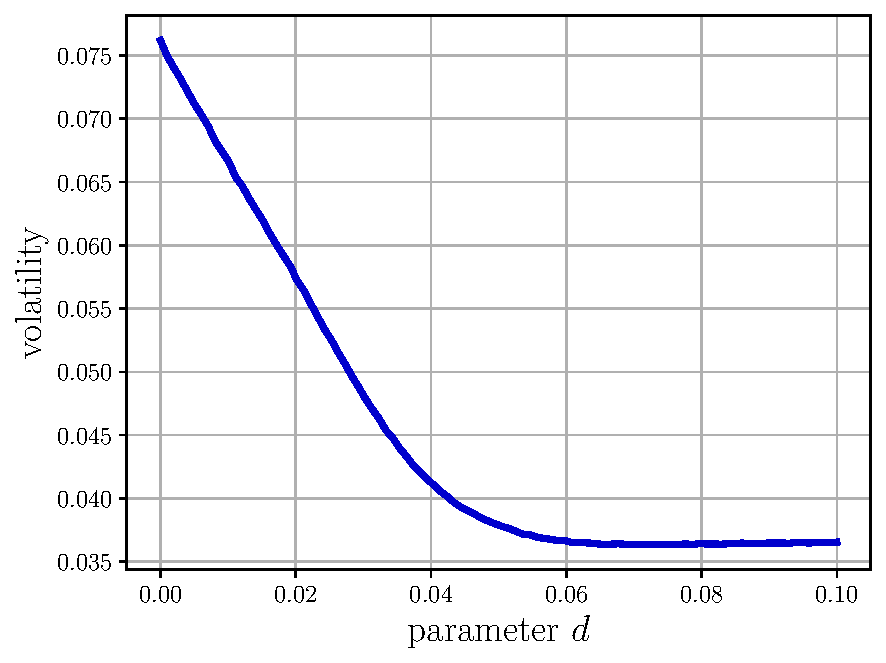
\includegraphics[width=0.4\textwidth]{../results/target-fundamental-volatility.pdf}\label{fig:a}}
	\hfil
	\sidesubfloat[]{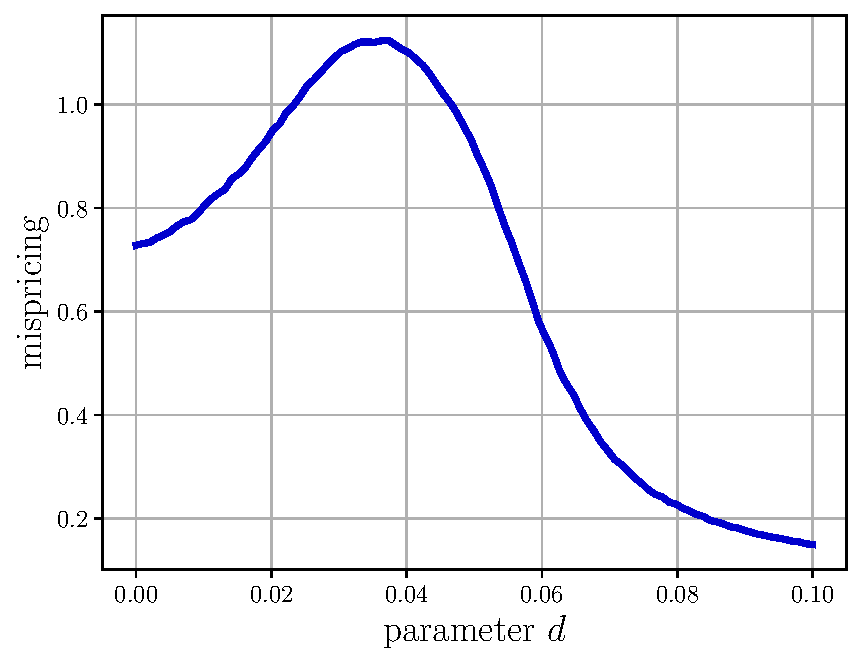
\includegraphics[width=0.4\textwidth]{../results/target-fundamental-mispricing.pdf}\label{fig:b}}
	
	\medskip
	\sidesubfloat[]{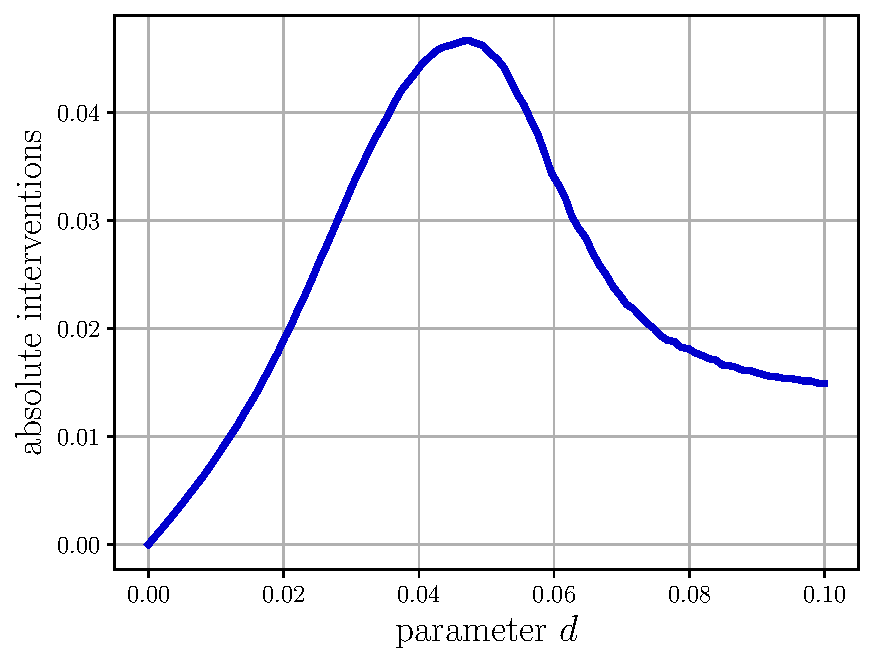
\includegraphics[width=0.4\textwidth]{../results/target-fundamental-absint.pdf}\label{fig:c}}
	\hfil
	\sidesubfloat[]{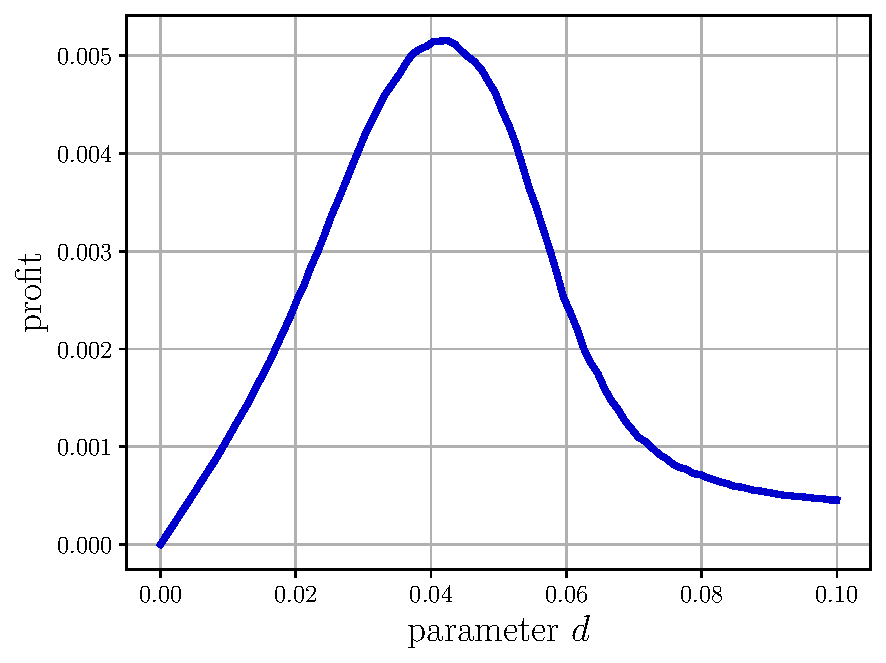
\includegraphics[width=0.4\textwidth]{../results/target-fundamental-profit.pdf}\label{fig:d}}
	
	\medskip
	\sidesubfloat[]{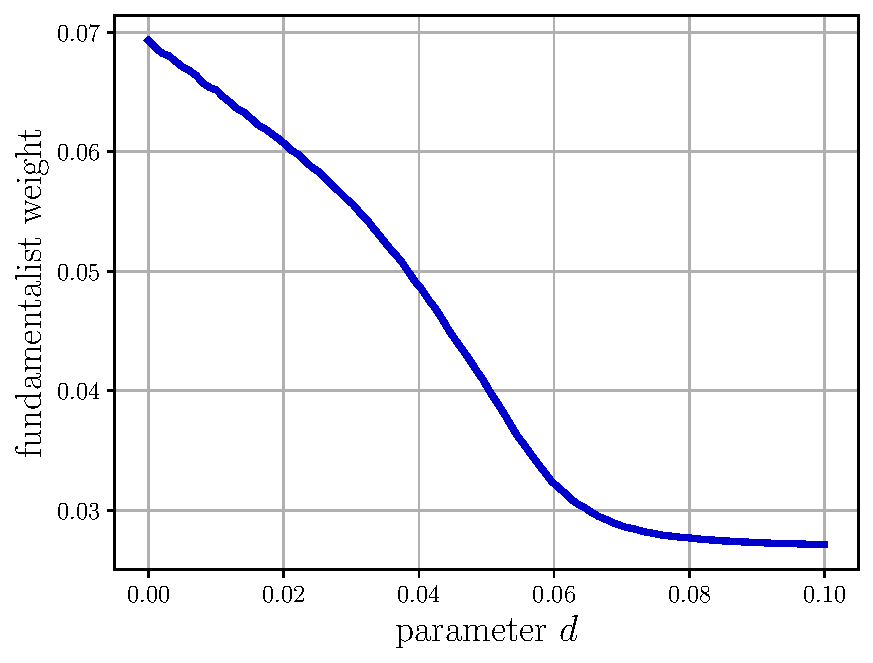
\includegraphics[width=0.4\textwidth]{../results/target-fundamental-fundweight.pdf}\label{fig:e}}
	\hfil
	\sidesubfloat[]{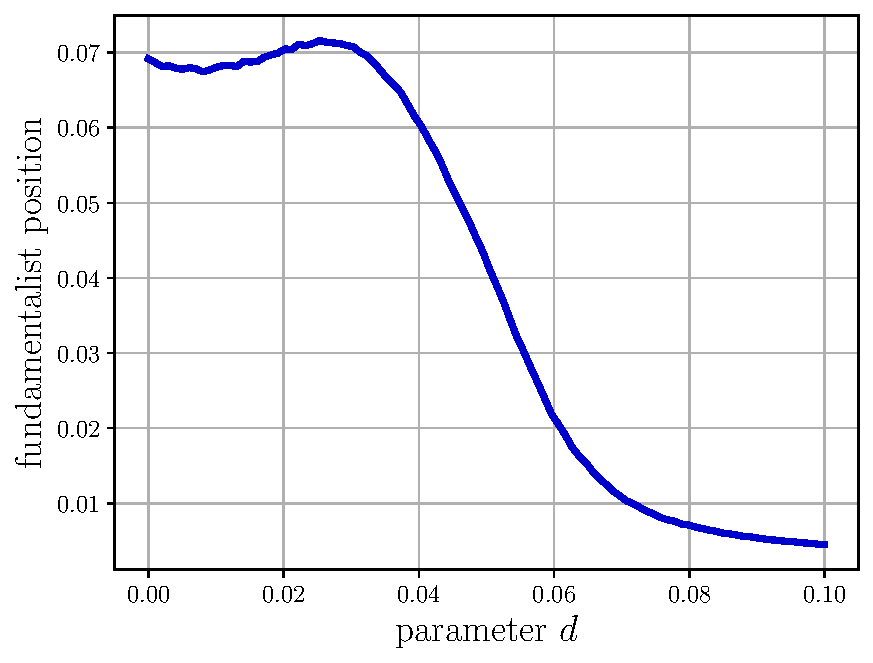
\includegraphics[width=0.4\textwidth]{../results/target-fundamental-fundpos.pdf}\label{fig:f}}
	\caption{تاثیر دخالت دولت در بازار}
	\label{fig:myfigure}
\end{figure}
شش سنجه تعریف شده در شکل ۶، اینجا نیز مورد بررسی قرار می‌گیرند تا صرفه و عملکرد استراتژی دولت را مورد بررسی قرار دهند. در قیاس با استراتژی قبلی دولت می‌توان گفت - از آنجا که تاثیرات مشابهی بین دو استراتژی داریم- چون پارامتر $m$ در حدود ده برابر $d$ مقیاس شده، پارامتر $d$ خیلی در کنترل موثرتر است(آ). از طرفی برخی مشکلات که در استراتژی اول بروز می‌داد اینجا بروز نمی‌دهد؛ مانند قیمت گذاری نادرست و حجم دخالت در بازار که در این استراتژی با افزایش پارامتر کنترل کاهش خواهد یافت(ب و ج). هم چنین چون دیگر استراتژی خلاف جهت بازار نیست، برای قانون گذار سود آور خواهد بود(د). از آنجا که بازار به قیمت بنیادی نزدیک می‌شود سودی در بنیادگرا بودن وجود نخواهد داشتو به همین دلیل تعداد آن‌ها کاهش خواهد داشت.






	\begin{figure}[H]
	\centering
	\sidesubfloat[]{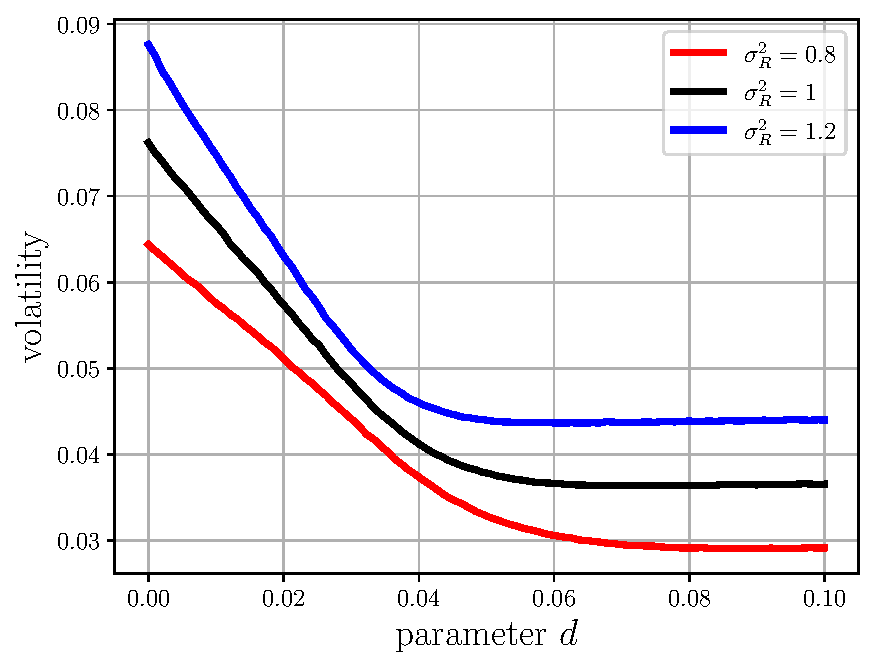
\includegraphics[width=0.4\textwidth]{../results/robust-belief-volatility.pdf}\label{fig:a}}
	\hfil
	\sidesubfloat[]{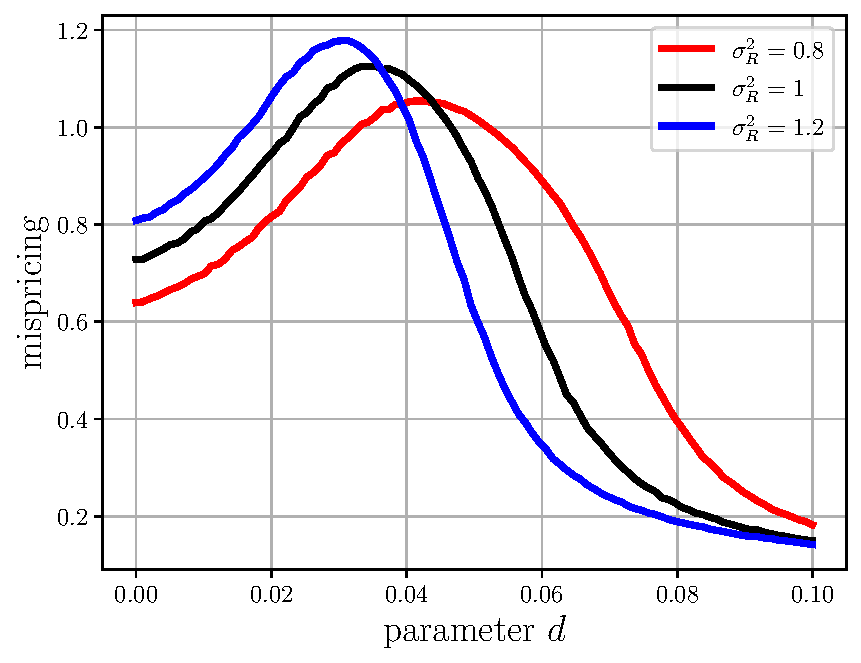
\includegraphics[width=0.4\textwidth]{../results/robust-belief-mispricing.pdf}\label{fig:b}}
	
	\medskip
	\sidesubfloat[]{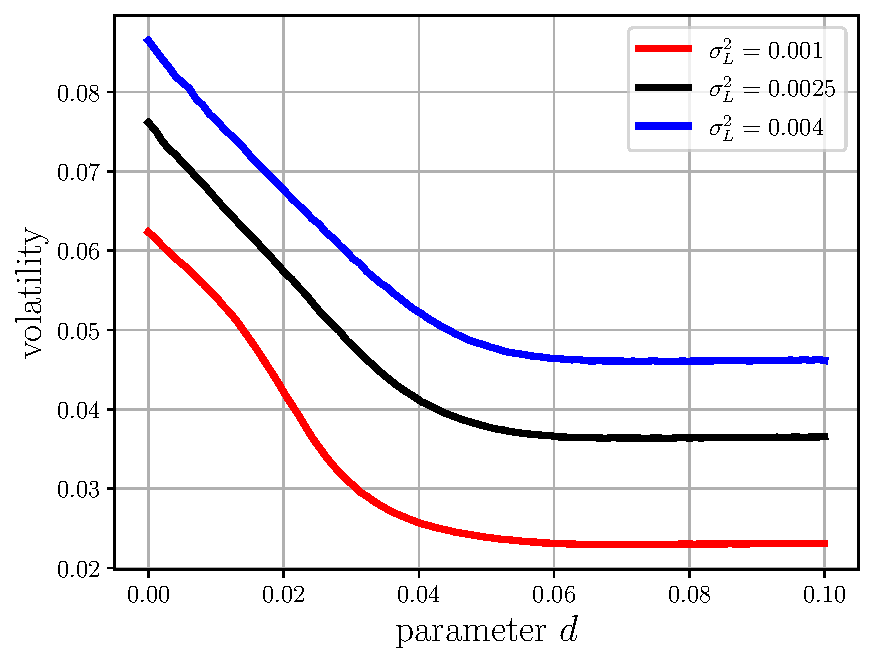
\includegraphics[width=0.4\textwidth]{../results/robust-randtrade-volatility.pdf}\label{fig:c}}
	\hfil
	\sidesubfloat[]{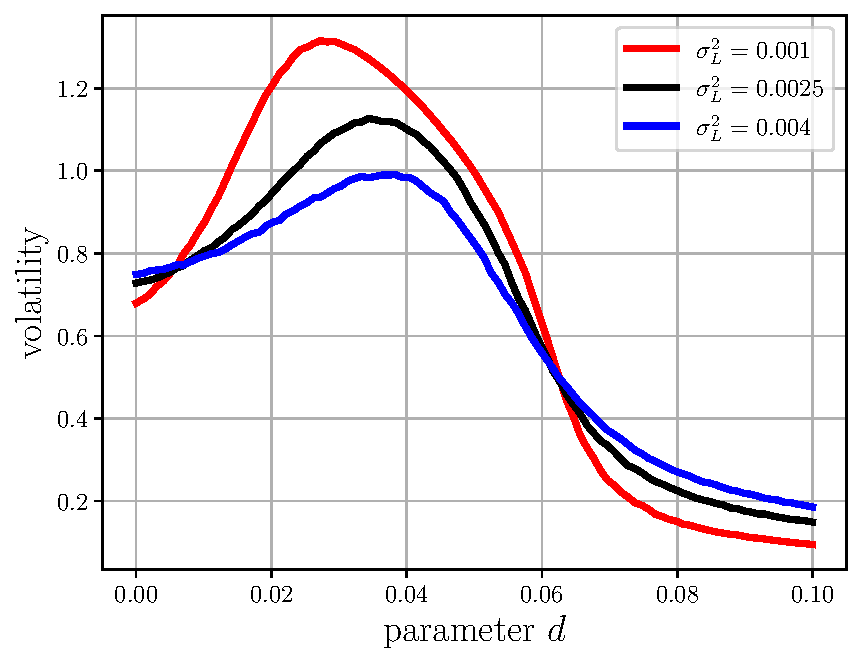
\includegraphics[width=0.4\textwidth]{../results/robust-randtrade-mispricing.pdf}\label{fig:d}}
	
	\medskip
	\sidesubfloat[]{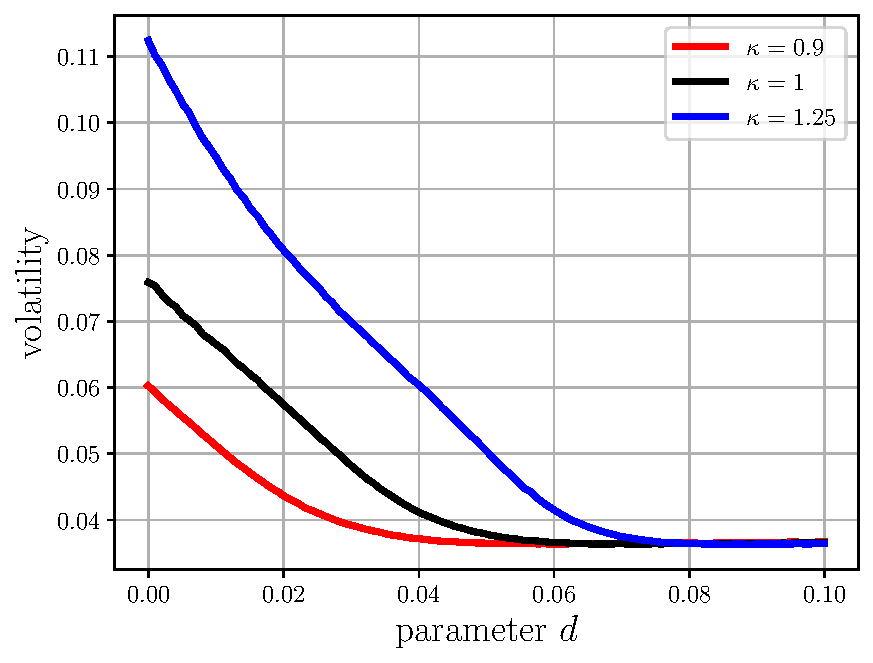
\includegraphics[width=0.4\textwidth]{../results/robust-fundcost-volatility.pdf}\label{fig:e}}
	\hfil
	\sidesubfloat[]{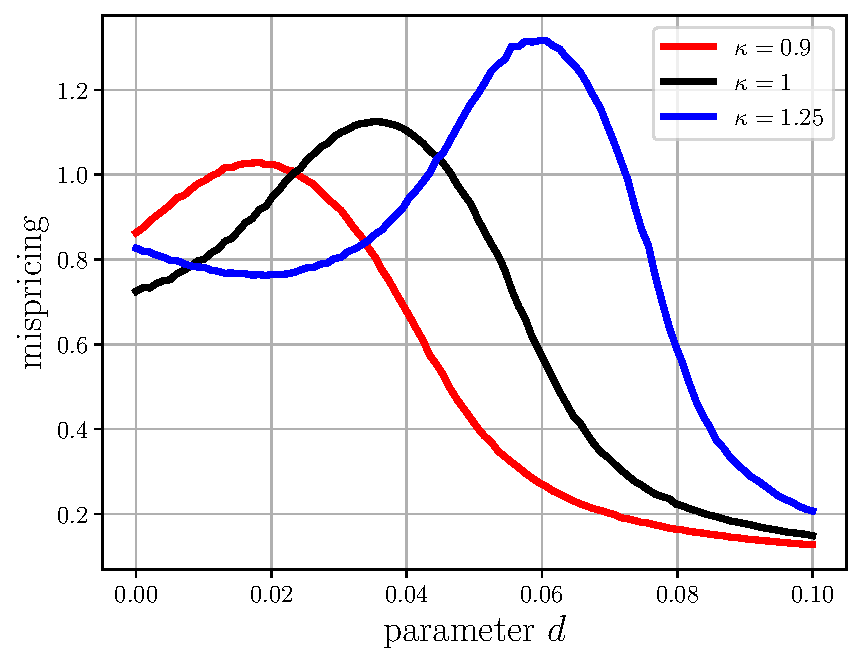
\includegraphics[width=0.4\textwidth]{../results/robust-fundcost-mispricing.pdf}\label{fig:f}}
	\caption{تاثیر پذیری استراتژی‌ها از پارامترهای مدل}
	\label{fig:myfigure}
\end{figure}
می‌خواهیم مقاومت سیاست‌های اجرایی را نسبت به تغییر پارامترها بررسی کنیم؛ اینکه آیا با تغییر پارامترهای مسئله باز هم این سیاست‌ها پاسخگو خواهند بود یا نه؟ با توجه به نمودارهای ترسیم شده می‌توان ادعا کرد که بله. این سیاست‌ها به ازای مقدایر مختف پارامترهای سیستم پاسخگو خواهند بود.



\section{جمع‌بندی}
مدلی که به بررسی آن پرداختیم با وجود آنکه بسیار ساده بود باز هم رفتار آشوبناک از خود بروز می‌داد. این رفتارها در واقعیت برای یک سیستم اقتصادی بسیار مخرب‌اند. از طرفی اینگونه رفتارها تنها در مدل‌های غیر خطی قابل مشاهده و بررسی اند به همین جهت این مدل‌ها برای قانون‌گذار قابل استفاده است تا بتوانند قوانین را قبل از وضع بیازمایند و تاثیر آن‌ها را بررسی کنند. به طور مثال در مدل مذکور مشاهده شد که استراتژی خرید (فروش) به هنگام کاهش (افزایش) قیمت در رخداد دوشاخگی‌ها بی تاثیر است اما از طرفی استراتژی هدایت قیمت به سمت قیمت بنیادی استراتژی کارآمدی برای کنترل این بازار بود.





	
\end{document}